\chapter{\hpc Supplementary Material}
\begin{table*}[h!]
\centering
\caption{Pairwise $C_{hyper}$ statistic for population comparisons.}
\begin{tabular}{@{}llll@{}}
\toprule
population 1 & population 2 & $C_{hyper}$   & $p$  \\ \midrule
US   & MH   & 3.82 & 1.11E-04 \\
US   & GH   & 6.17 & 8.00E-10 \\
MH   & GH   & 4.37 & 1.24E-05 \\
US   & AN   & 3.51 & 3.37E-04 \\
MH   & AN   & 2.73 & 4.43E-03 \\
GH   & AN   & 3.16 & 1.16E-03 \\ \bottomrule
\end{tabular}
\label{tab:C_hyper}
\end{table*}

% \hspace{2em}
\begin{table*}[h]
\centering
\caption[Selection outliers simultaneously detected in PBE and pcadapt analysis]{\textbf{Selection outliers simultaneously detected in PBE and pcadapt analysis}. These phosphoglycerolipid metabolism genes are in the top 5\% of Mexican highlands PBE, and are also in the top 5\% of significance ($-log_{10}(P)$) for the association with \textit{pcadapt} PC1 (elevation correlated principal component).  Further populations where the gene is an outlier for PBE are listed as well, maximum PBE  population is highlighted in bold.
}
\resizebox{\textwidth}{!}{%
\begin{tabular}{@{}ll@{ }l@{ }l@{ }lllrrll@{}}
\toprule
               & \multicolumn{5}{c}{\textbf{PBE}}                             & \multicolumn{3}{c}{\textbf{pcadapt}} &                                                                                                        &                                                                                                  \\
\cmidrule(lr){2-6} \cmidrule(lr){7-9}  
Gene           & \multicolumn{4}{c}{Outlier Population}      & Max  & chr   & bp          & \textbf{$-log_{10}(P)$}   & Description                                                                                            & Example Pathway                                                                                  \\
\midrule
Zm00001d009280 &             & \textbf{MH} &    &             & 0.55 & 8     & 50352267    & 207.55                    & \begin{tabular}[c]{@{}l@{}}phosphoethanolamine\\ N-methyltransferase\end{tabular}                      & \begin{tabular}[c]{@{}l@{}}superpathway of phospholipid \\ biosynthesis II (plants)\end{tabular} \\
Zm00001d046915 &             & MH          & GH & \textbf{AN} & 0.81 & 9     & 107790977   & 138.64                    & AMP-dependent synthetase                                                                               & phosphatidylcholine acyl editing                                                                 \\
Zm00001d014425 &             & \textbf{MH} & GH &             & 1.19 & 5     & 44991886    & 134.29                    & Glycerol-3-phosphate acyltransferase                                                                   & \begin{tabular}[c]{@{}l@{}}superpathway of phospholipid\\ biosynthesis II (plants)\end{tabular}  \\
\underline{Zm00001d039542} & US          & \textbf{MH} & GH &             & 1.01 & 3     & 8542287     & 110.28                    & \begin{tabular}[c]{@{}l@{}}Phospholipase A1-Igamma1 chloroplastic\\ HPC1\end{tabular}                  & phosphatidylcholine acyl editing                                                                 \\
\underline{Zm00001d017584} & \textbf{US} & MH          & GH & AN          & 0.86 & 5     & 195455216   & 99.31                     & \begin{tabular}[c]{@{}l@{}}Lysophospholipid acyltransferase 1\\ ZmLPCAT1\end{tabular}                  & phosphatidylcholine acyl editing                                                                 \\
Zm00001d040629 & US          & MH          & \textbf{GH} & AN          & 1.80 & 3     & 55167339    & 85.67                     & Lysophospholipid acyltransferase LPEAT1                                                                &                                                                                                  \\
Zm00001d043267 & \textbf{US} & MH          &    &             & 1.11 & 3     & 190926980   & 68.94                     & \begin{tabular}[c]{@{}l@{}}acyl-CoA:1-acyl-sn-glycerol-3-phosphate \\ 2-O-acyltransferase\end{tabular} & \begin{tabular}[c]{@{}l@{}}superpathway of phospholipid\\ biosynthesis II (plants)\end{tabular}  \\
Zm00001d043263 &             & \textbf{MH} & GH & AN          & 1.02 & 3     & 190792965   & 66.70                     & Diacylglycerol kinase 5                                                                                & \begin{tabular}[c]{@{}l@{}}phosphatidate metabolism,\\ as a signaling molecule\end{tabular}      \\ \bottomrule
\end{tabular}%
}
\label{tab:Sup:top_candidates}
\end{table*}
\clearpage

\begin{figure*}[t]
\begin{center}
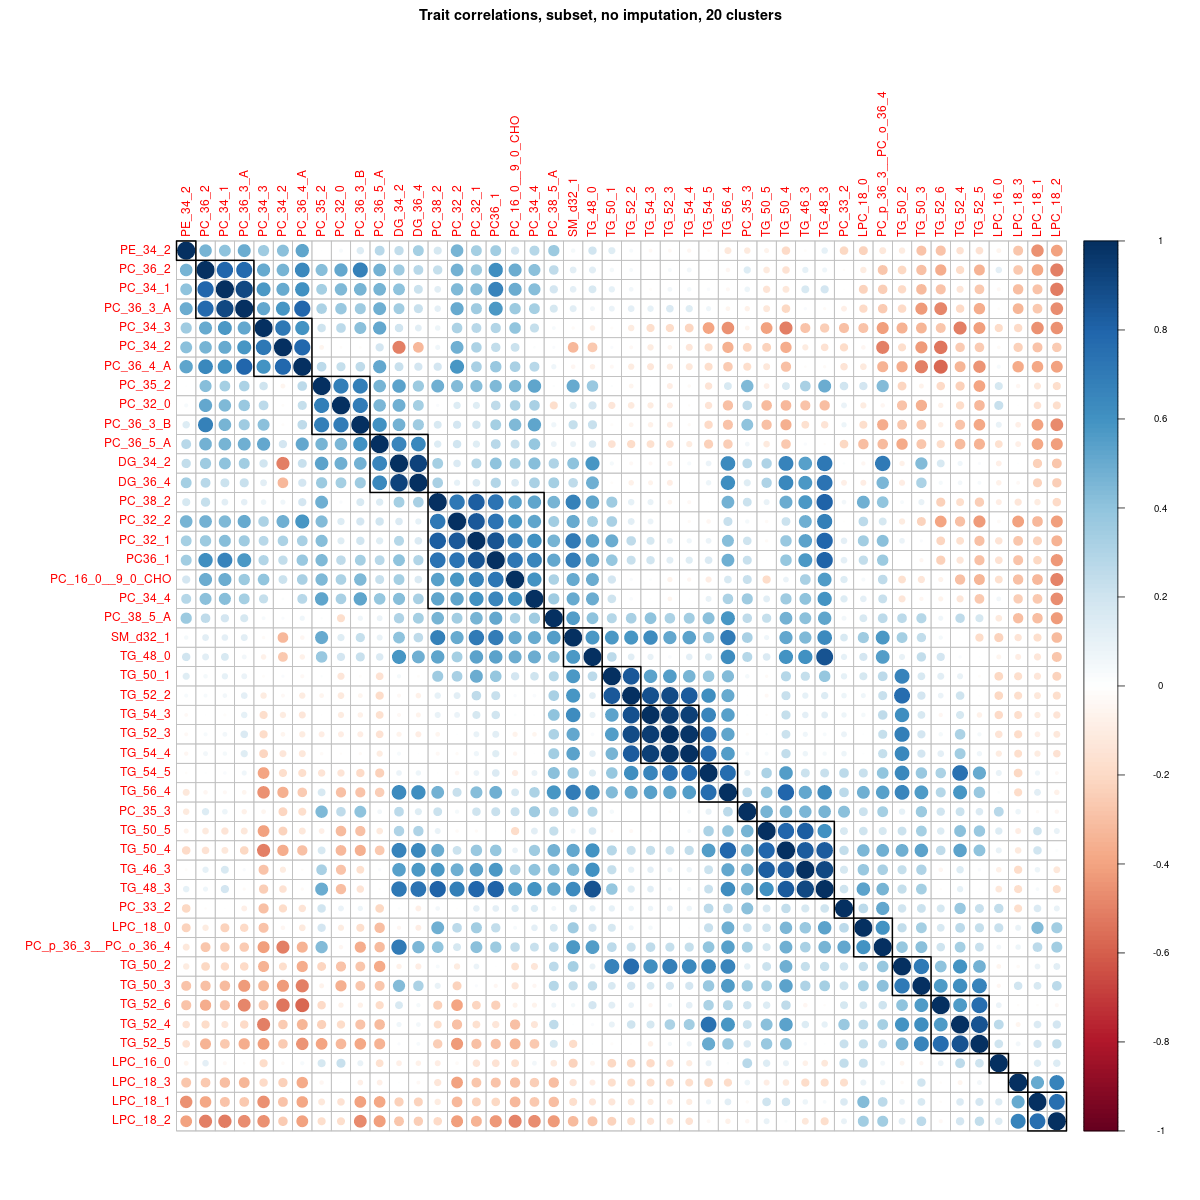
\includegraphics[width=\linewidth]{Sup_Figures/Sup_Fig_1.png}
\caption[Cluster analysis of lipidomics data]{\textbf{Cluster analysis of lipidomics data.} Representative species from each cluster were used for $Q_{ST}$-$F_{ST}$ analysis}
\label{figure:Sup:lipid_clusters}
\end{center}
\end{figure*} 
\clearpage

\begin{figure*}[t]
\begin{center}
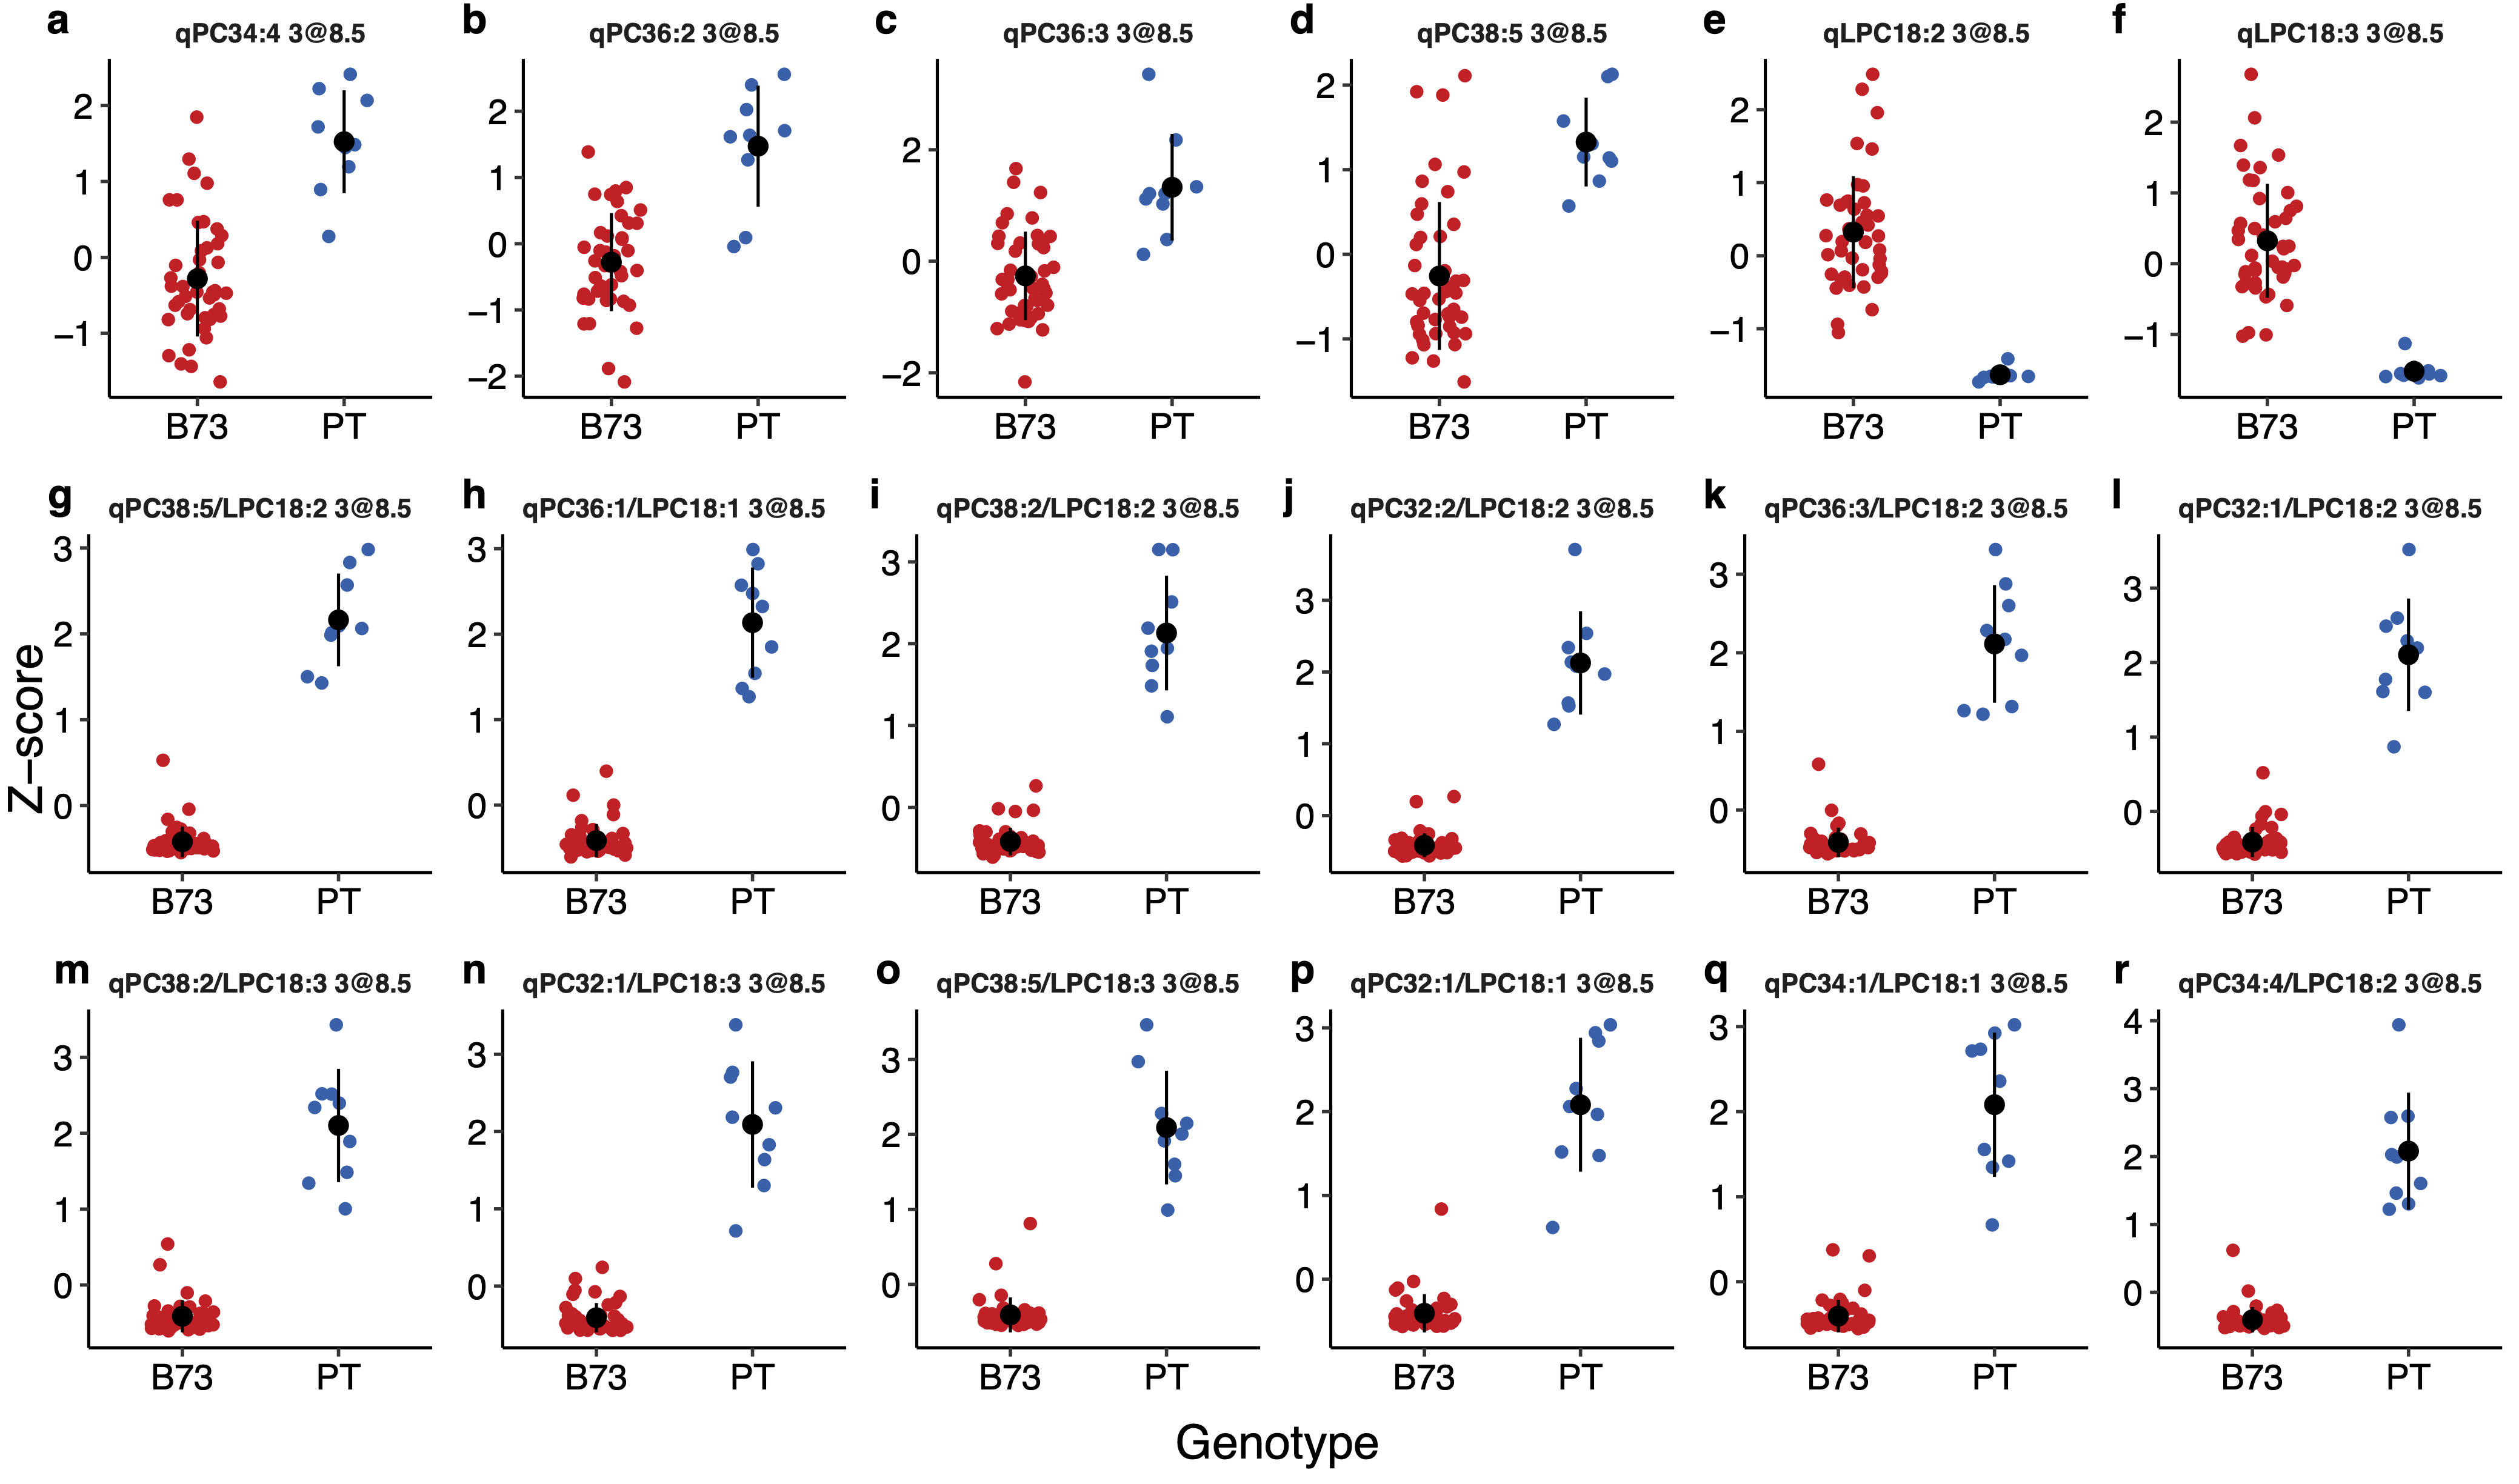
\includegraphics[width=\linewidth]{Sup_Figures/Sup_Fig_2.png}
\caption[Effects of QTLs at chromosome 3 @8.5 Mb]{\textbf{Effects of QTLs at chromosome 3 @8.5 Mb} \textbf{(a-d)} Effect for individual PC \textbf{(e-f)} and LPC species
\textbf{(g-r)} The 12 most significant peaks for PC/LPC ratios} 
%\label{QTL_effect_sp}
\label{figure:Sup:QTL_effect_sp}
\end{center}
\end{figure*}  
\clearpage

\begin{figure}[t]
\begin{center}
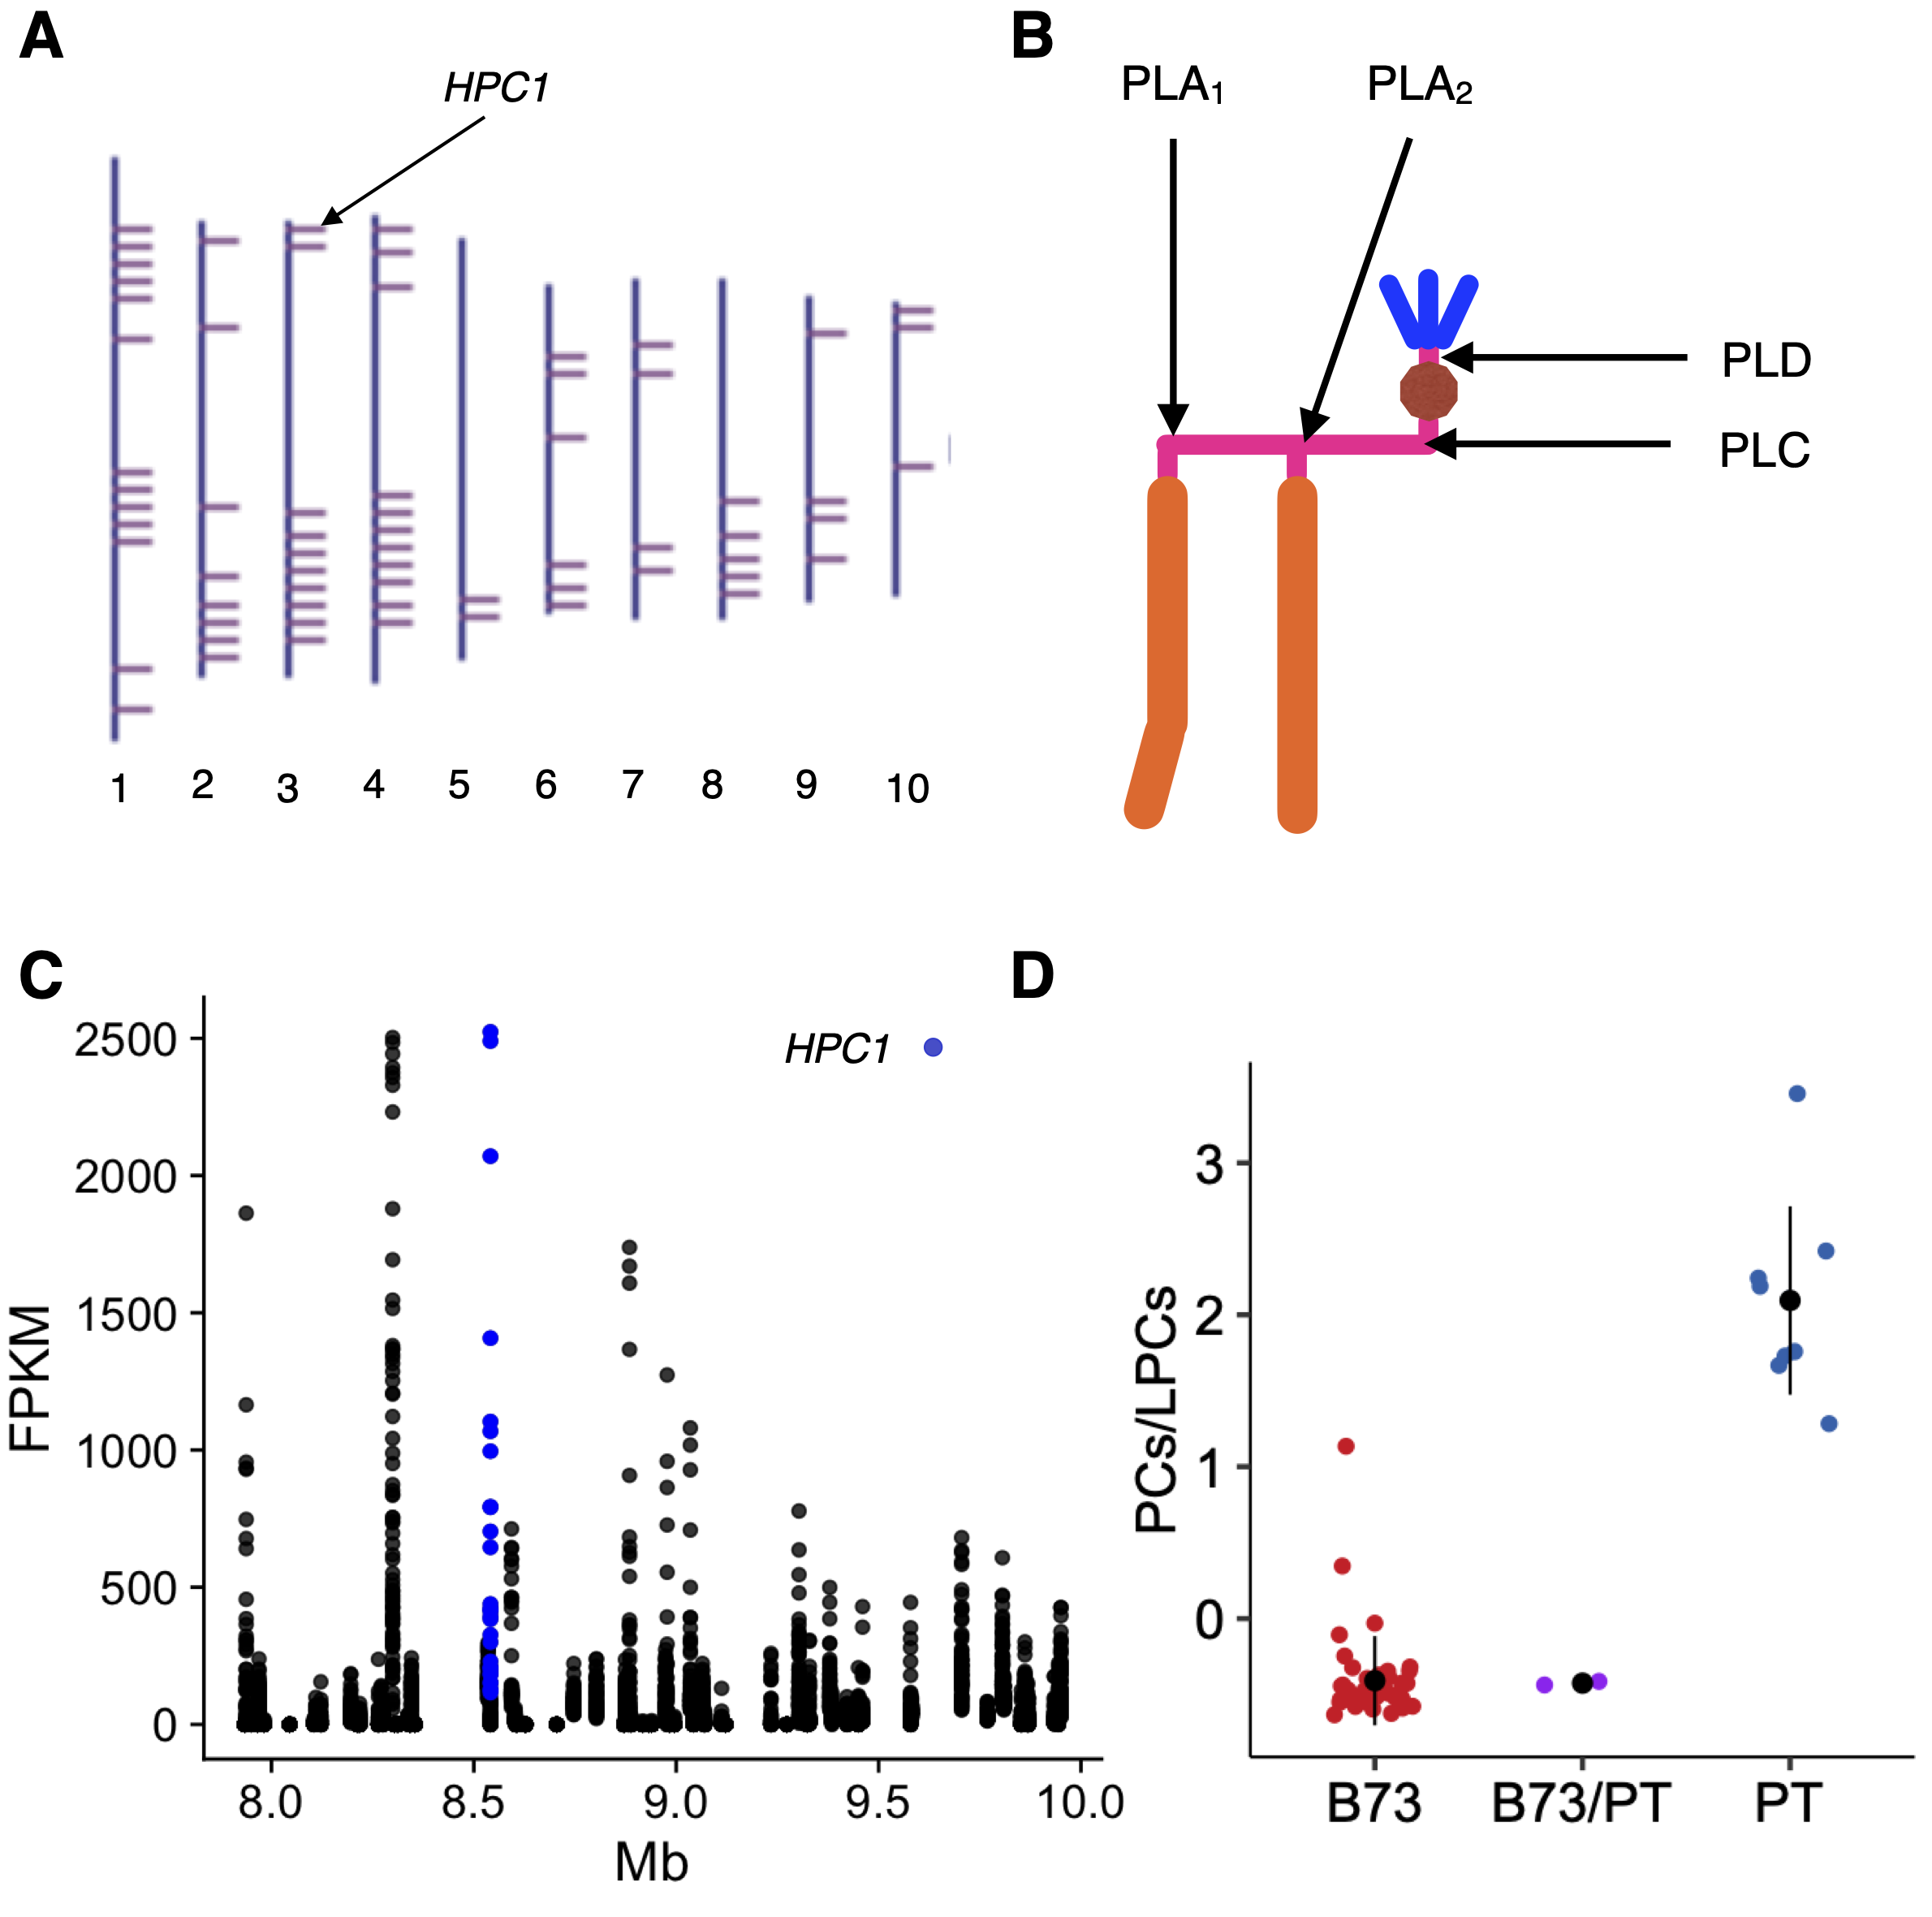
\includegraphics[width=\linewidth]{Sup_Figures/Sup_Fig_3.png}
\caption[Phospholipase activity in maize.]{\textbf{Phospholipase activity in maize.} \textbf{(A)} Genomic location of genes encoding proteins with predicted phospholipase A1 activity. 
\textbf{(B)} Site of action of the different types of phospholipases.
\textbf{(C)} Expression levels from B73 leaves for genes in the 7.9--10 Mb QTL interval of chromosome 3. Data from \cite{stelpflug2016-vr}
\textbf{(D)} Effect sizes of PC/LPC levels at RILs homozyzogous for B73, PT or heterozygous at the QTL qPC/LPC3@8.5.
}
\label{figure::Sup:HPC1_misc}
\end{center}
\end{figure} 
\clearpage

\begin{figure*}[t]
\begin{center}
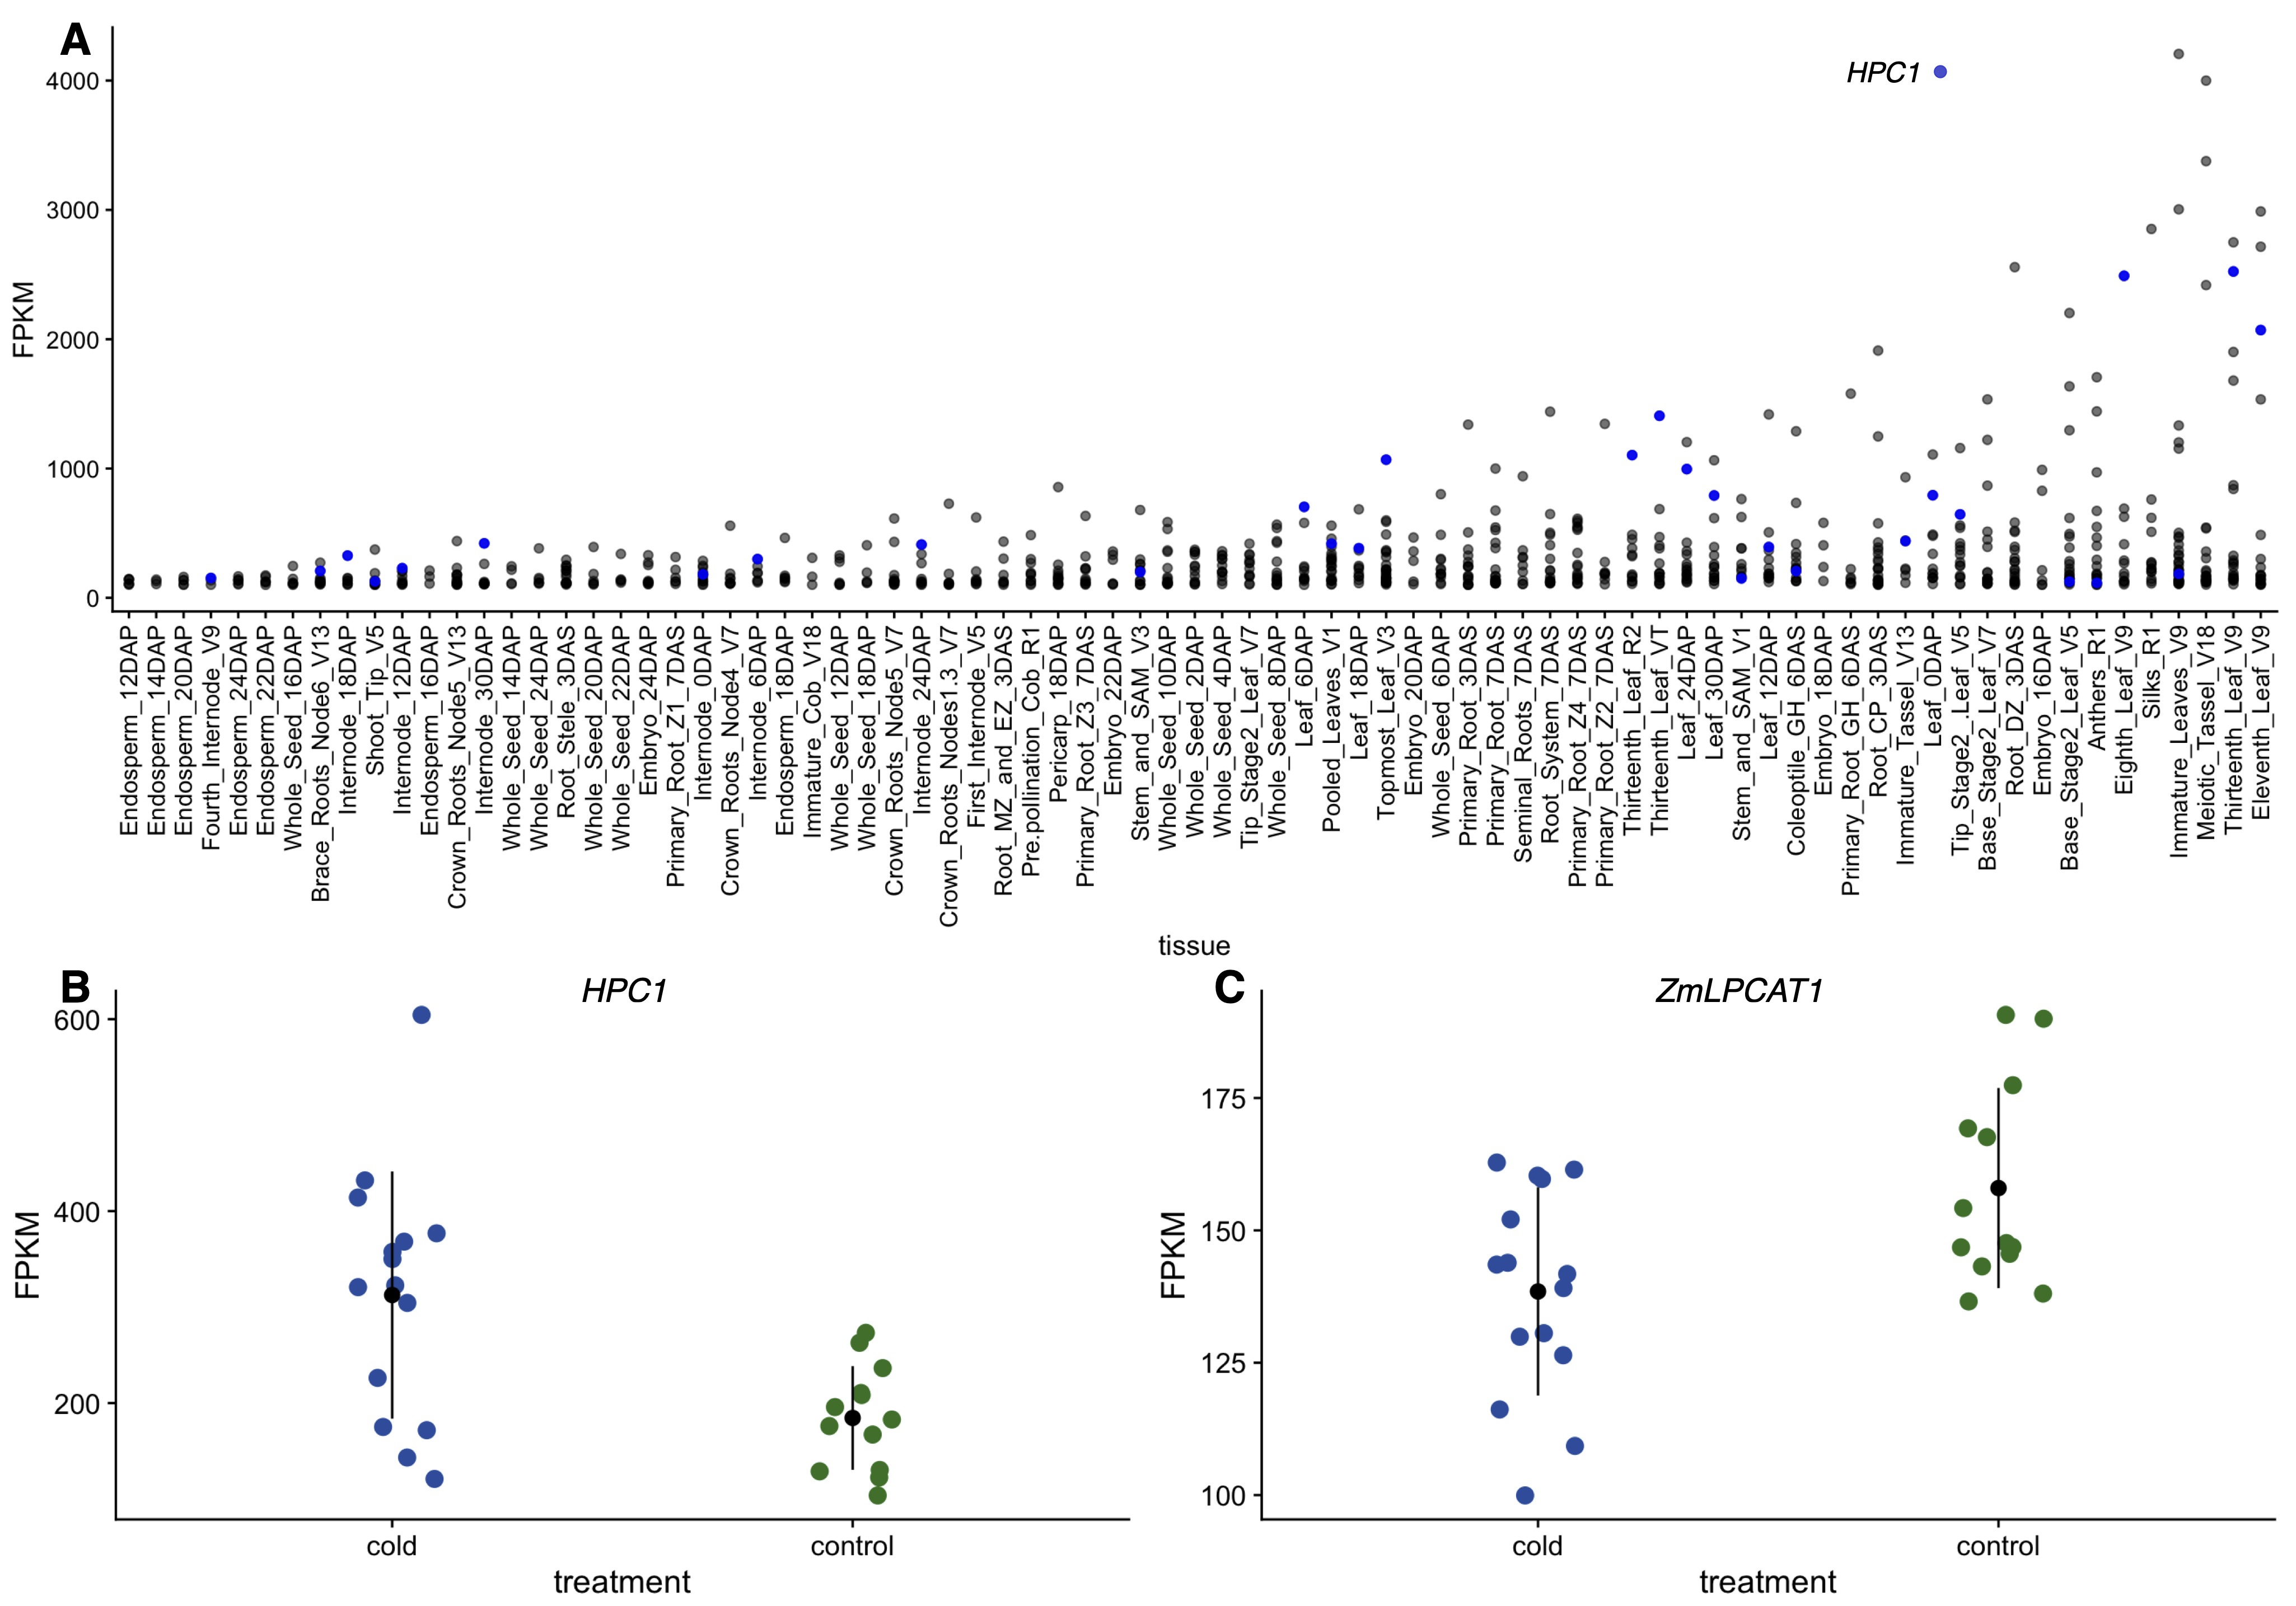
\includegraphics[width=\linewidth]{Sup_Figures/Sup_Fig_4.png}
\caption[Phospholipase expression in temperate inbred lines.]{\textbf{Phospholipase expression in temperate inbred lines.} \textbf{A)} Expression levels in B73 of genes encoding enzymes with predicted phospholipase A1 activity across different tissues. \hpc is indicated in blue. 
Data from \cite{stelpflug2016-vr}.
\textbf{B)}  and \textbf{C)}\hpc and \textit{ZmLPCAT1} expression levels in the temperate inbred lines B73, Mo17, OH43, and PH207 under cold and control conditions. Values taken from \cite{waters2017-nat}).
}
\label{figure:Sup:B73_expression}
\end{center}
\end{figure*} 
\clearpage

\begin{figure}[t]
\begin{center}
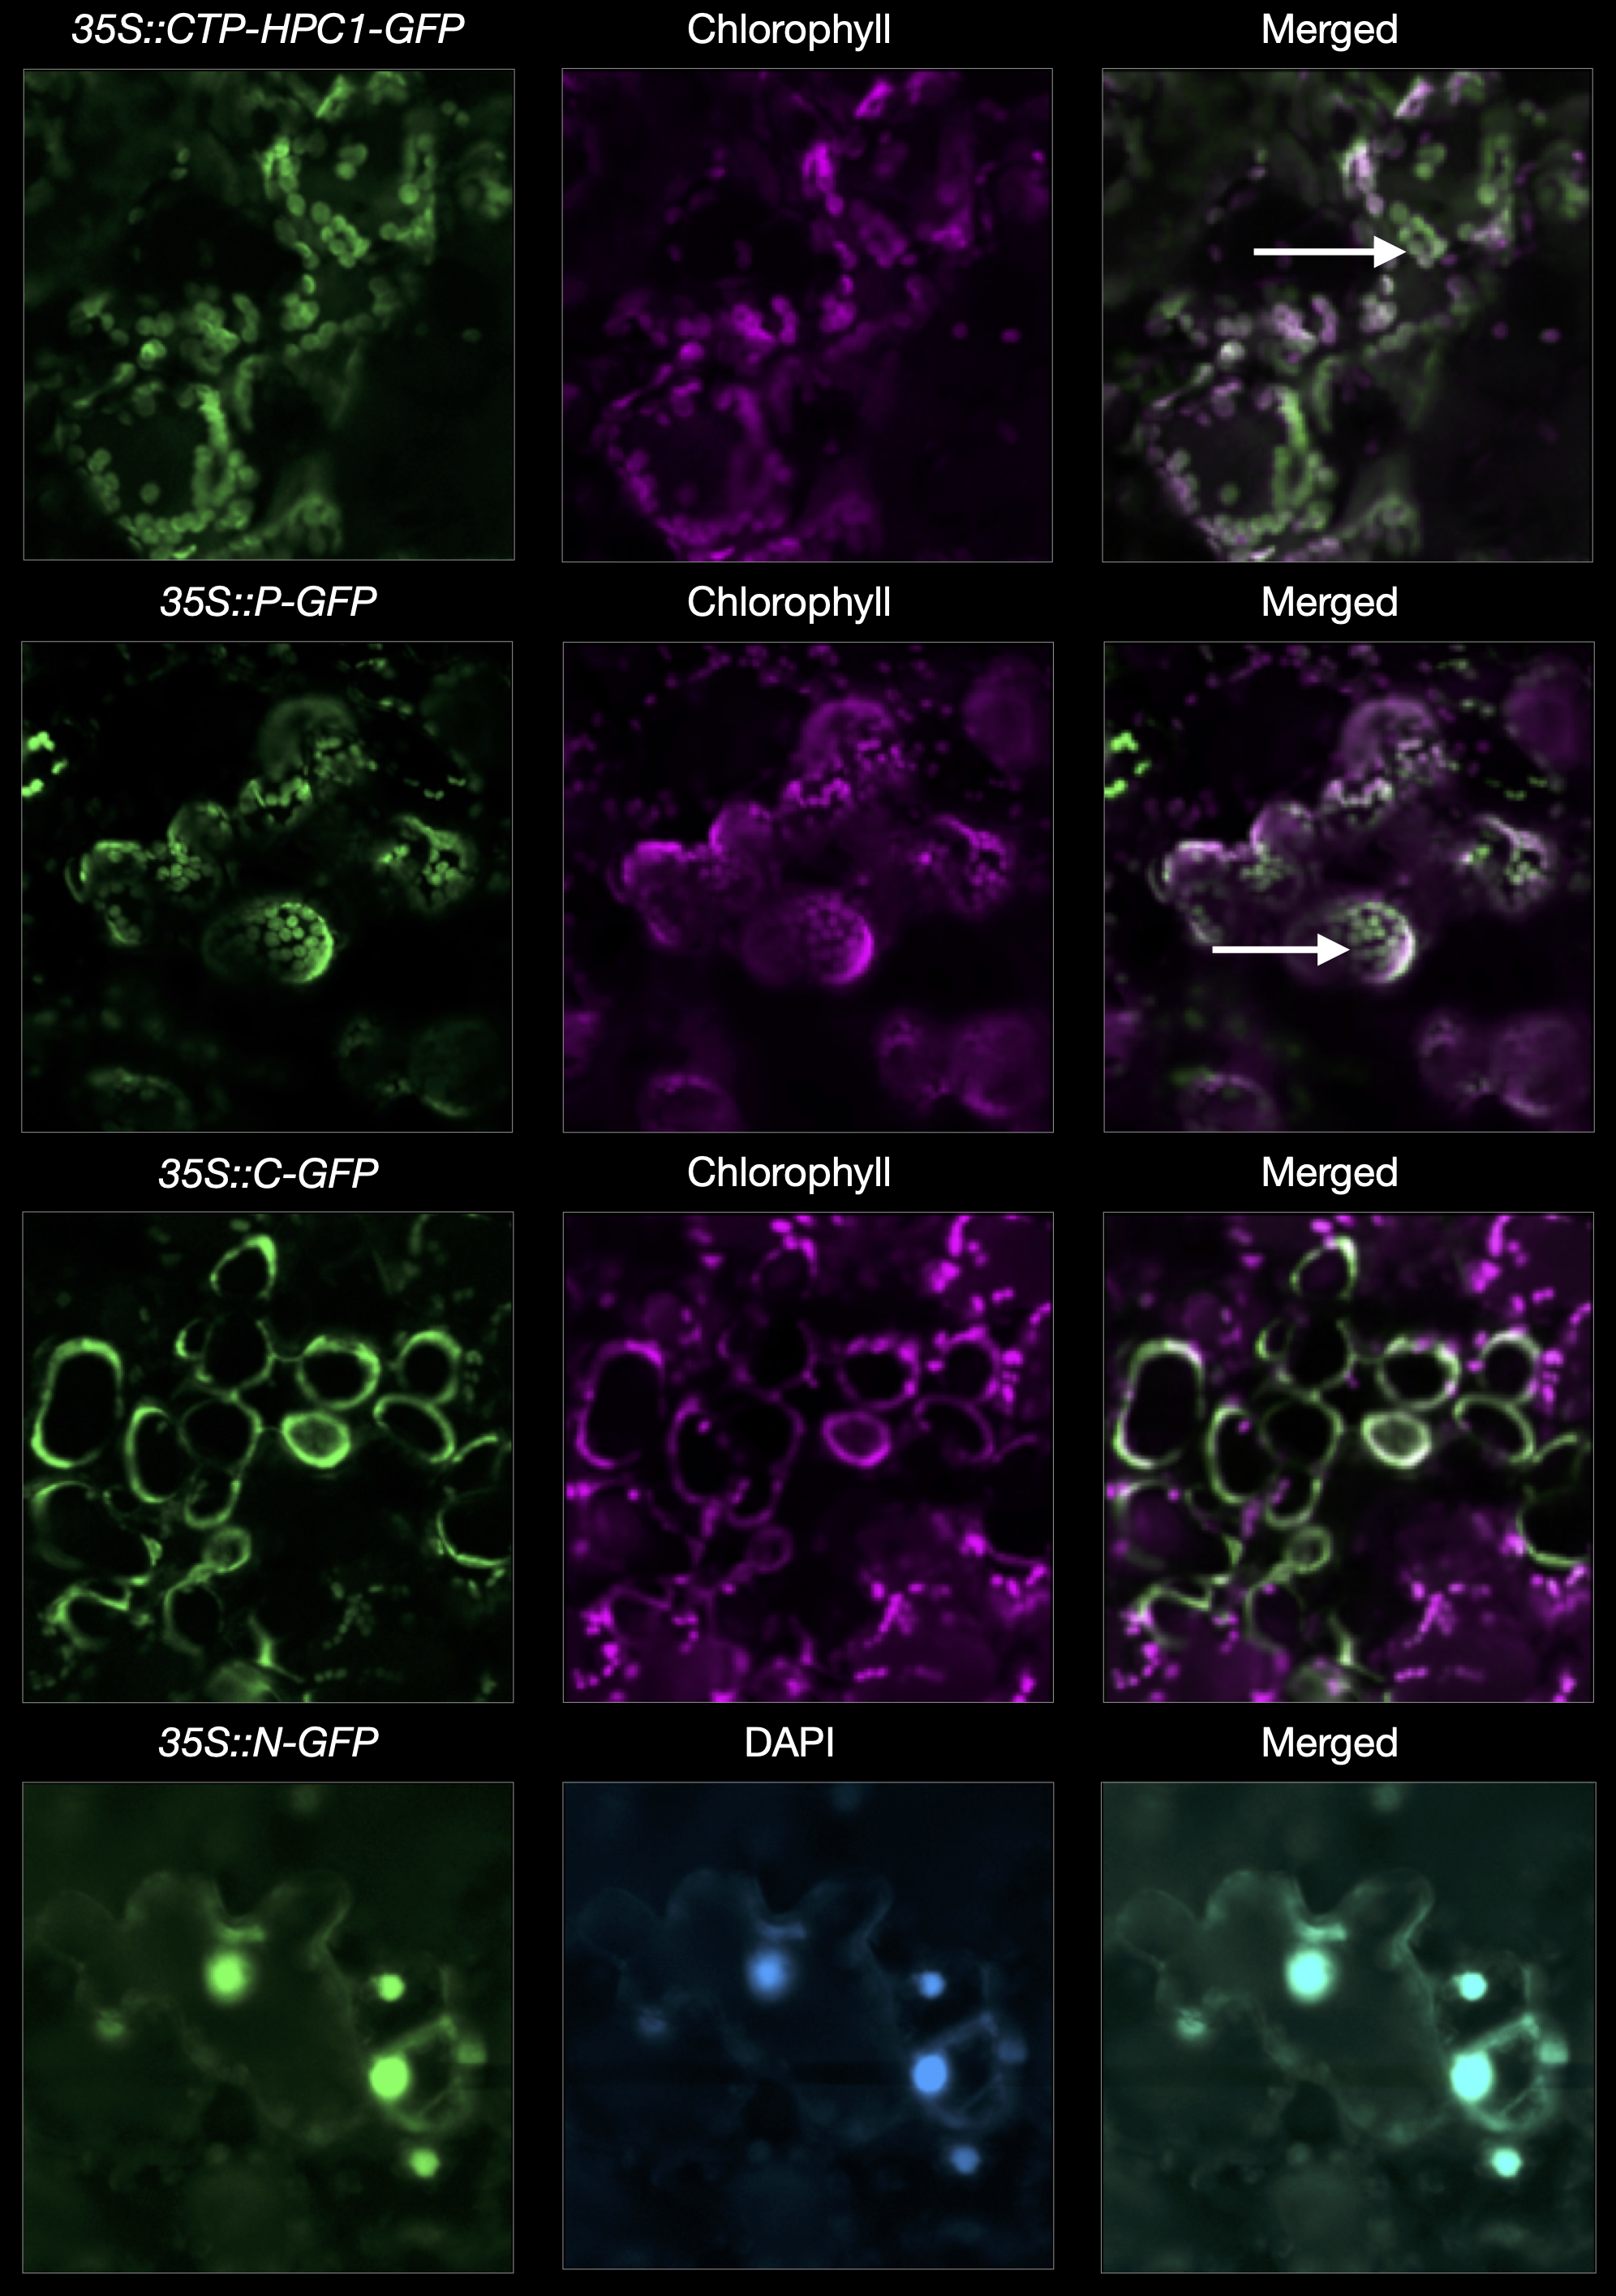
\includegraphics[width=0.8\linewidth]{Sup_Figures/Sup_Fig_5.png}
\caption[Subcellular localization of HPC1 in \textit{Nicotiana benthamiana} epidermal leaf cells.]{\textbf{Subcellular localization of HPC1 in \textit{Nicotiana benthamiana} epidermal leaf cells.}   
CTP.HPC1-GFP, corresponding to the first 52 amino acids HPC1, were fused to GFP. 
Three constructs for various subcellular compartments were used as control; cytoplasm (C-GFP), nucleus (N-GFP), and chloroplast (P-GFP). All reporters were under the control of the cauliflower Mosaic Virus (CaMV) 35S promoter. The white arrows show chloroplast and nucleus.
} 
\label{figure:Sup:HPC1_organelle}
\end{center}
\end{figure} 
\clearpage

\begin{figure*}[t]
\begin{center}
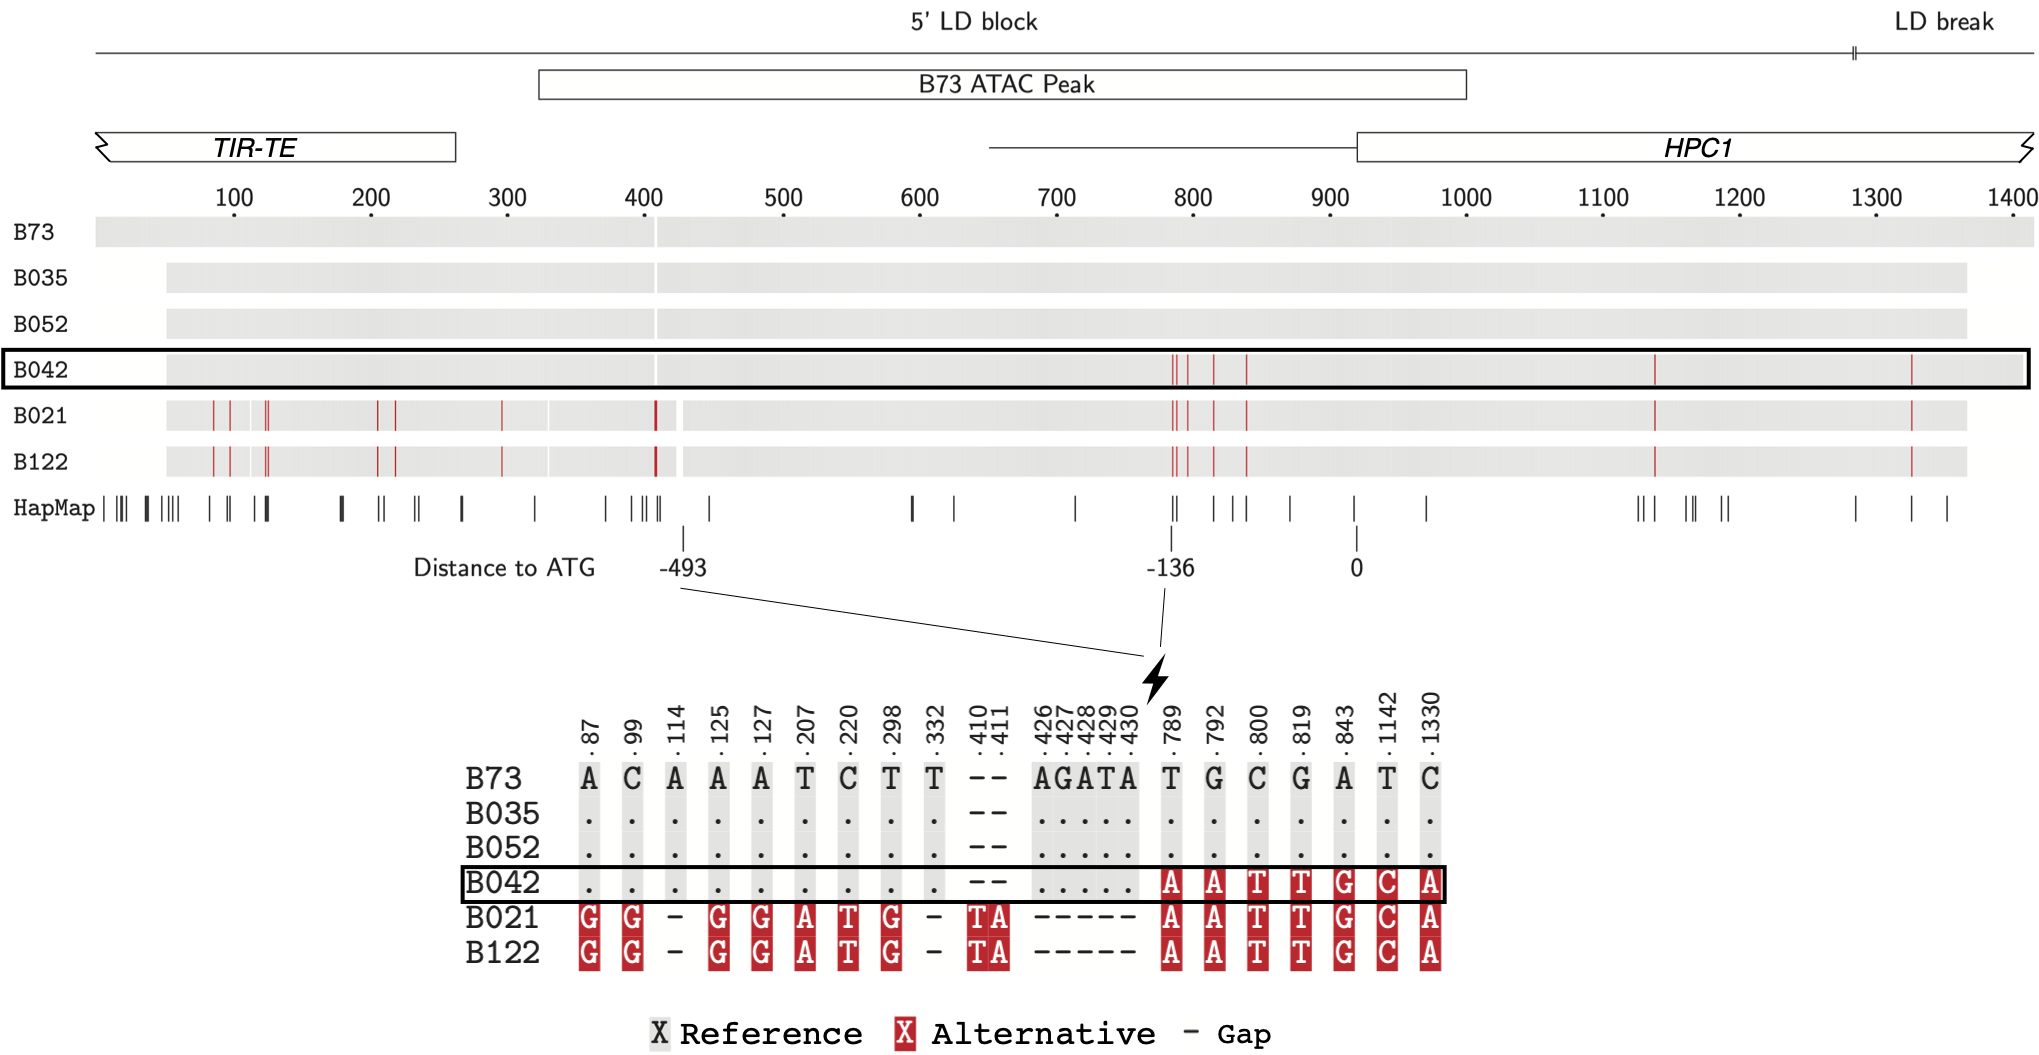
\includegraphics[width=\linewidth]{Sup_Figures/Sup_Fig_6.png}
\caption[Recombination at the \hpc promoter in the B73 x PT segregating population.]{\textbf{Recombination at the \hpc promoter in the B73 x PT segregating population.} \textit{Overview (top)} 1419 bp global alignment of Sanger sequences from B73 and 5 RILs (B035, B052, B042, B021 and B122). At variant positions B042 shows B73 genotype (grey) up to alignment position 430, and PT genotype (red) from 789 downstream. We infer that there is  a recombination breakpoint between -493 and -136 bp upstream the translation start codon of B042.
HapMap track shows HapMap2.7 SNPs used for Linkage Disequilibrium calculations in MaizeSNPDB as in Figure 5. The 5' LD block spans the upstream intergenic region, including two ATAC-seq chromatin accessibility peaks (one included in this fragment), and up to 364 bp of \hpc coding sequence. 
Then there is a LD break, and a downstream 3' LD block (not included in these sequences). 
\textit{TIR-TE} terminal inverted repeat transposable element. 
B73 ATAC-seq: narrow peak showing chromatin accessibility in leaf tissue \cite{ricci2019-zj}.
\textit{Base pair detail (bottom)} B73 and and PT nucleotide alleles are marked in grey and red respectively.
Coordinate numbers on top of both views are global alignment positions.
}
\label{figure:Sup:hpc1_promoter}
\end{center}
\end{figure*}
\clearpage

\begin{figure*}[t]
\begin{center}
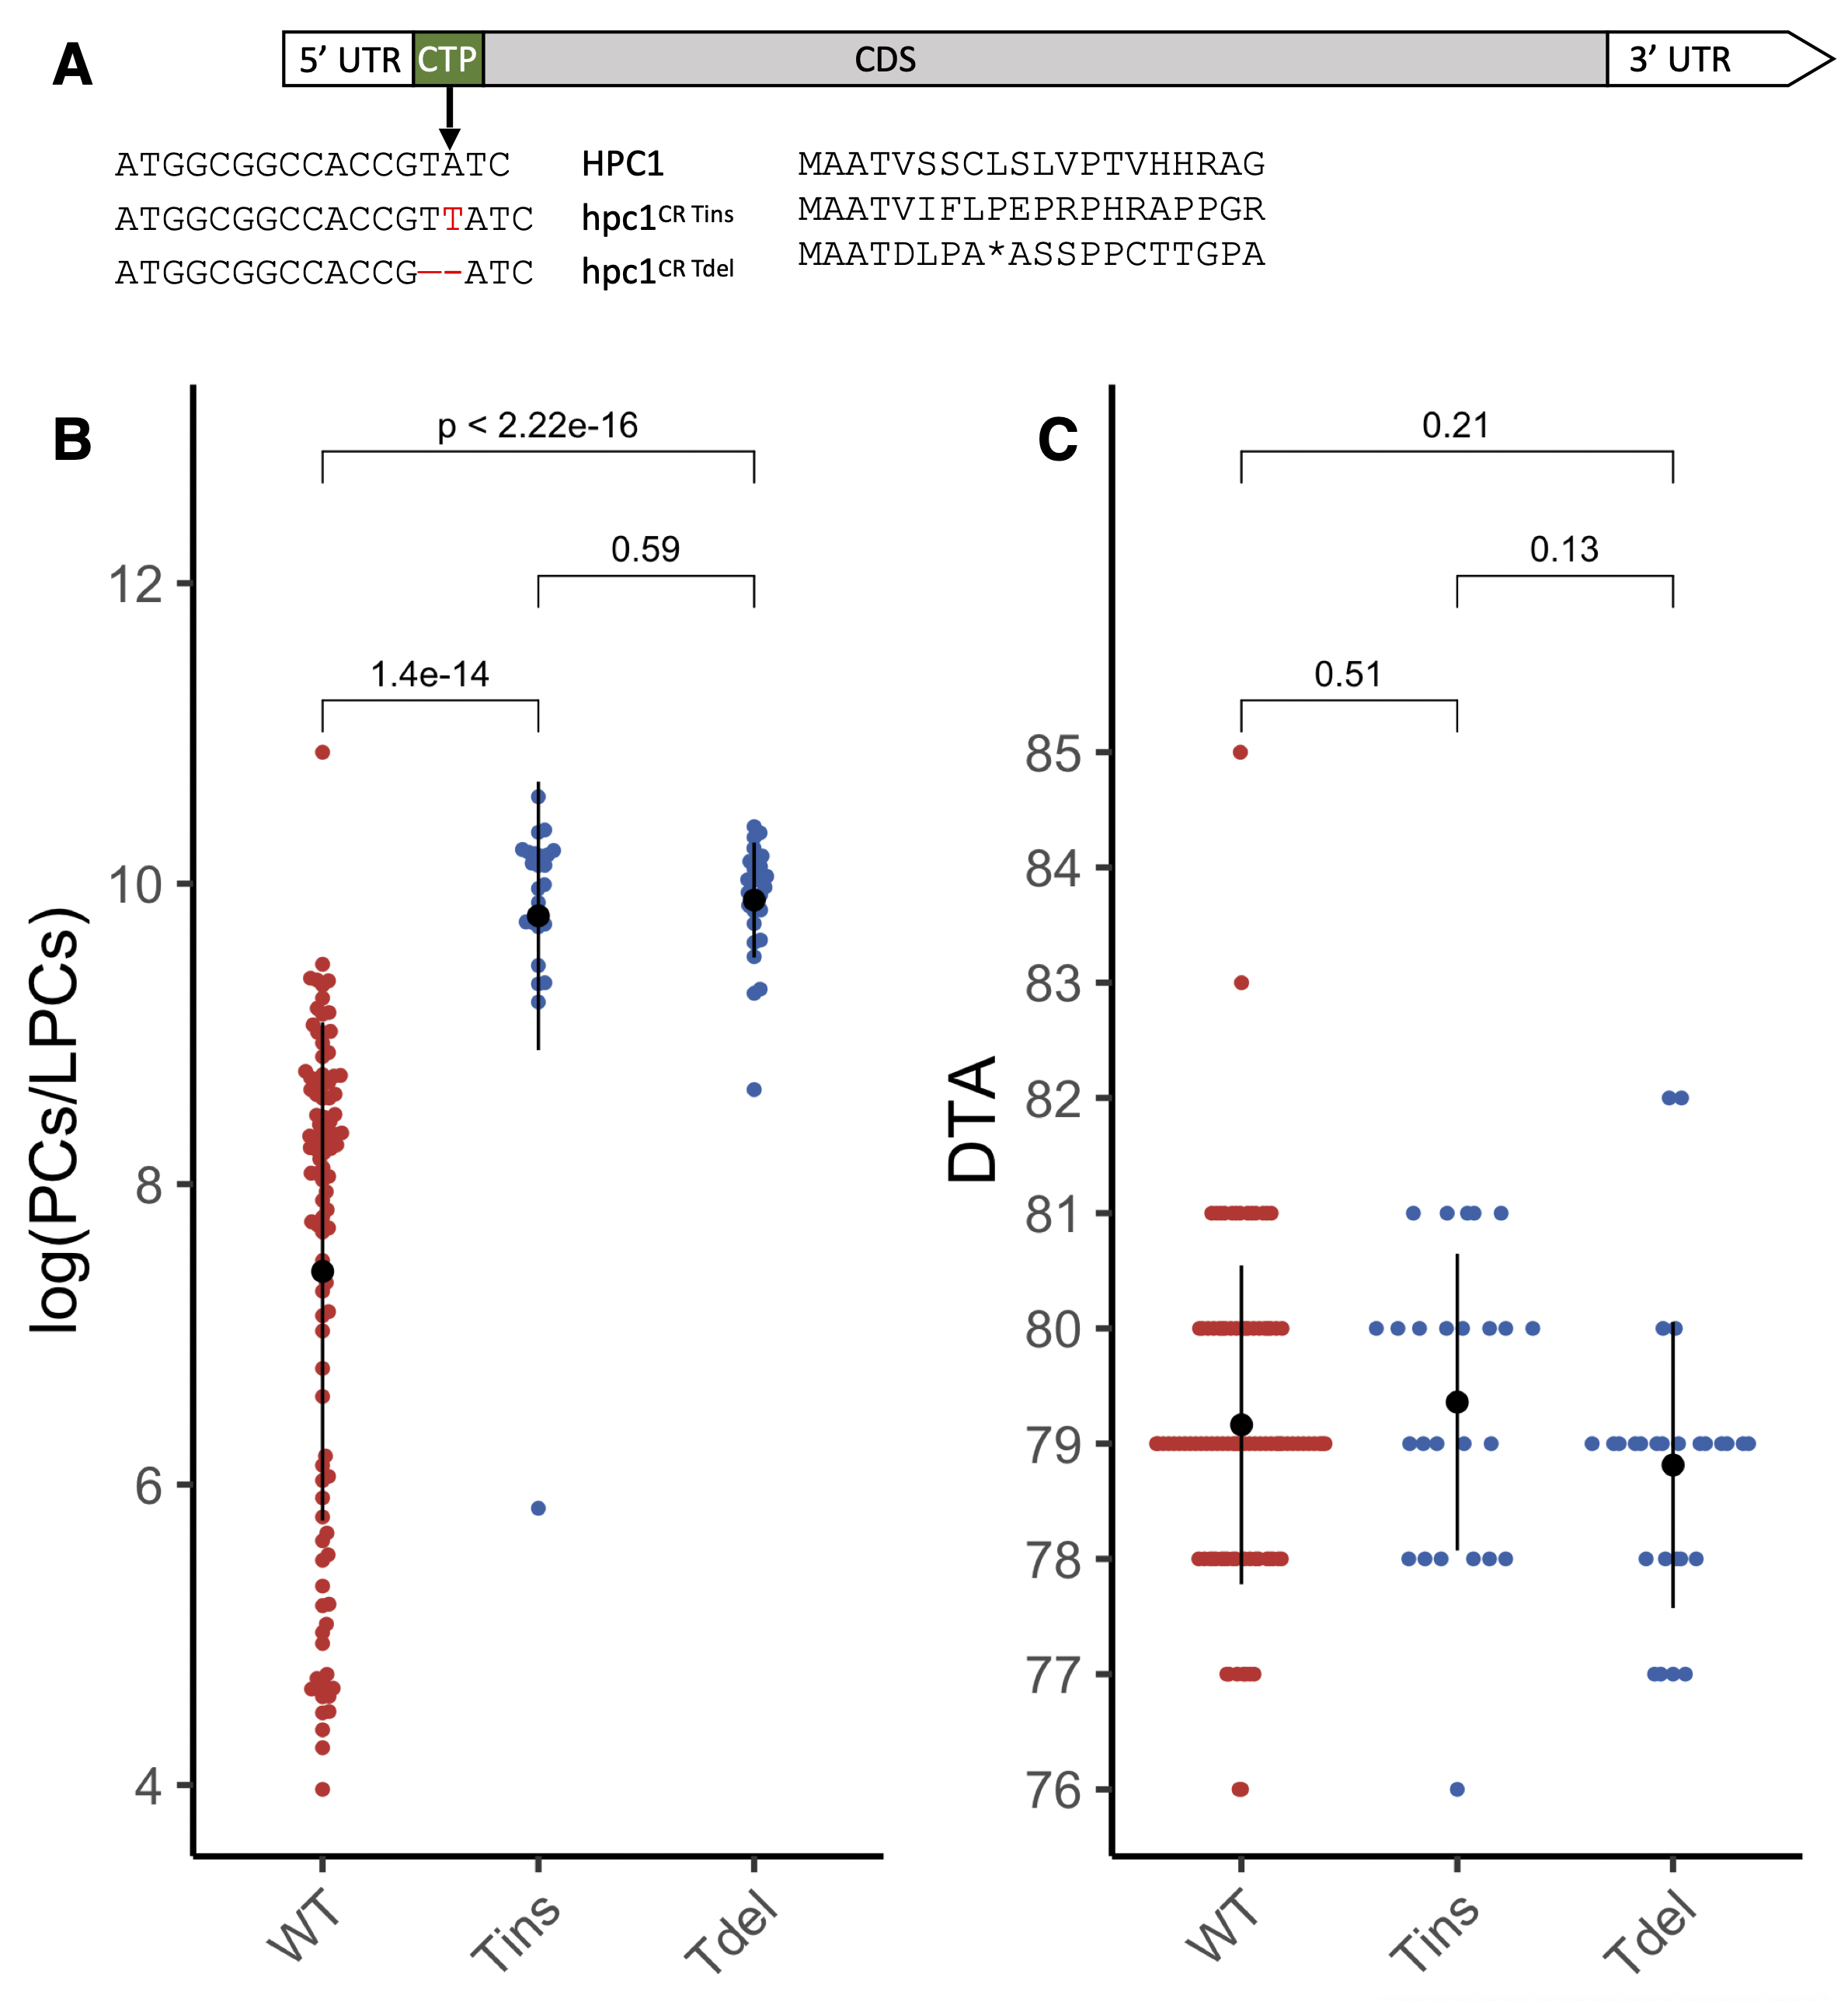
\includegraphics[width=0.8\linewidth]{Sup_Figures/Sup_Fig_7.png}
\caption[Effects of the \textit{hpc1\textsuperscript{CR}} allele.]
{\textbf{Effects of the \textit{hpc1\textsuperscript{CR}} allele.}
\textbf{(A)} Physical location of \hpc CRISPR mutant alleles. \textbf{(B)} log(PCs/LPCs) ratios of WT and the \hpc CRISPR mutant alleles. \textbf{(C)} Days to anthesis of the same plants shown in panel A.   
}
\label{figure:Sup:CRISPR_effect}
\end{center}
\end{figure*} 
\clearpage



\begin{figure*}[t]
\begin{center}
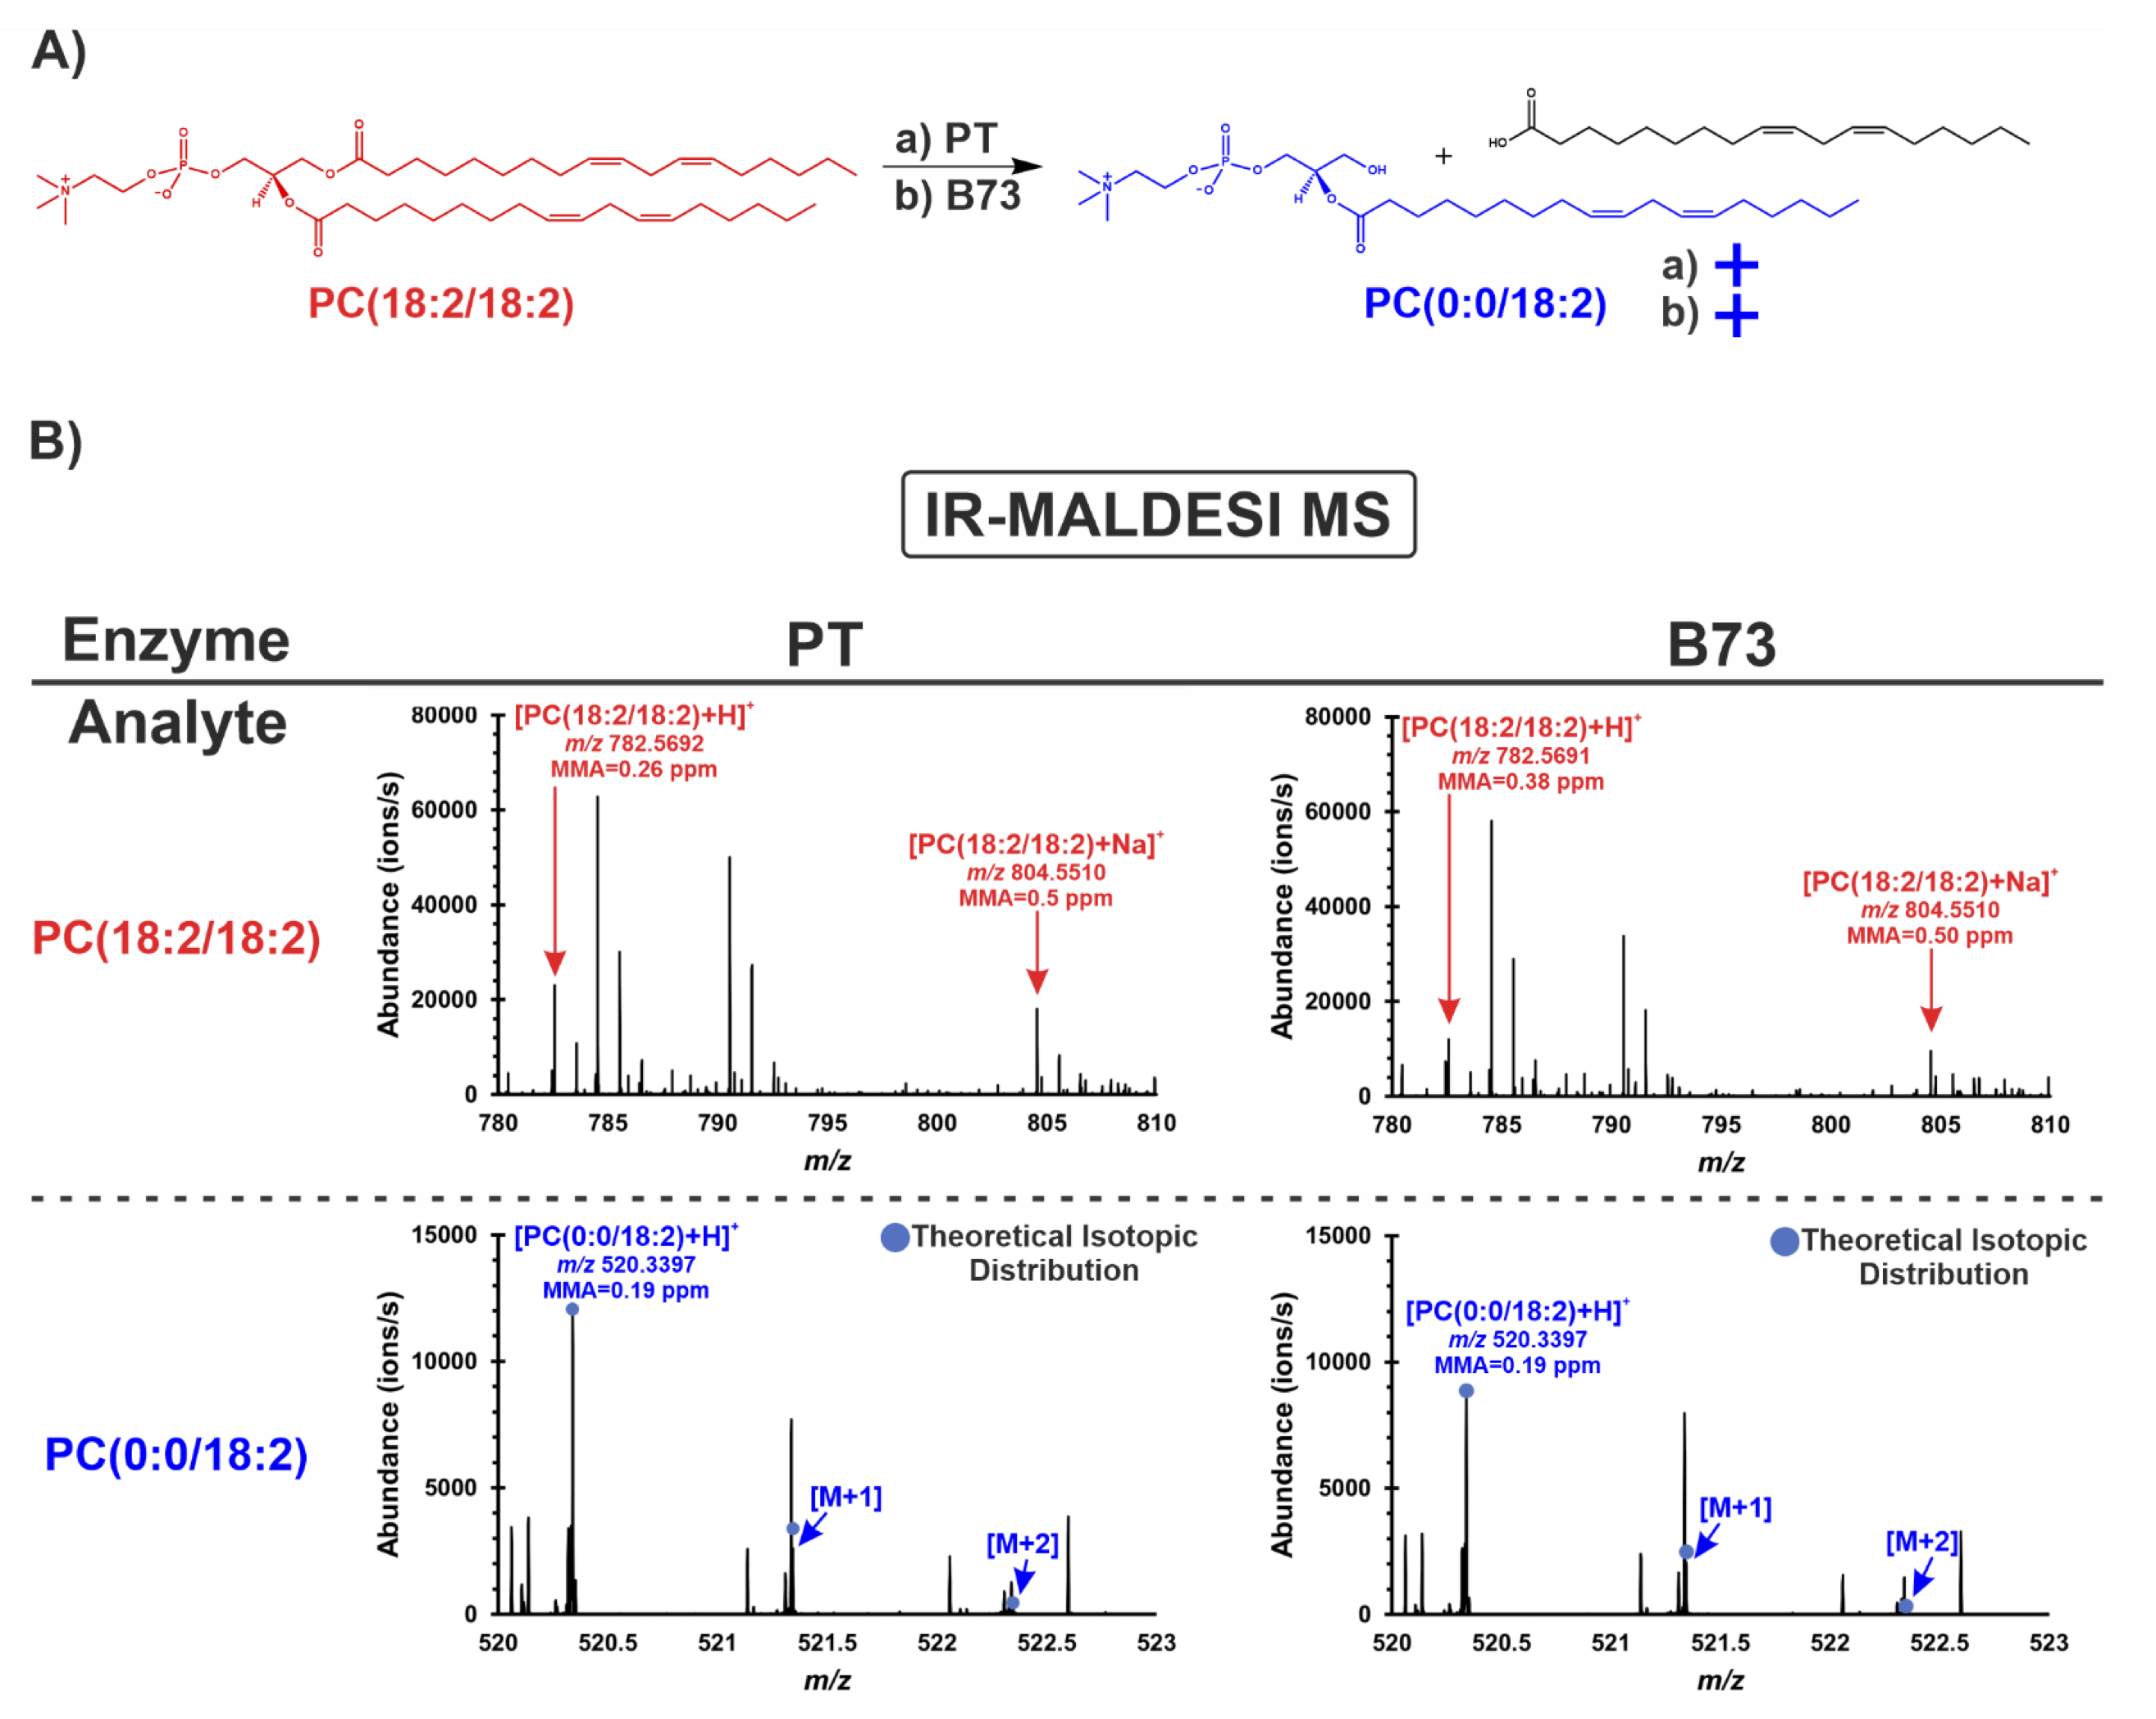
\includegraphics[width=\linewidth]{Sup_Figures/Sup_Fig_8.png}
\caption[\hpc alleles have phospholipase activity.]
{\textbf{\hpc alleles have phospholipase activity.}
\textbf{A} Schematic of the \hpc reaction of PC(18:2/18:2) (red) to
PC(0:0/18:2) (blue). 
\textbf{B} IR-MALDESI-MS mass spectra of the HPC1 reaction using the \textit{HPC1-PT} and \textit{HPC1-B73} alleles. The
experimental \textit{m/z} and mass measurement accuracy (MMA) is labelled below each
identification. 
Both protonated and sodiated adducts of PC(18:2/18:2) were measured. 
Each mass spectrum was averaged over 100 scans.}
\label{figure:Sup:MS_spectra}
\end{center}
\end{figure*} 
\clearpage

\begin{figure*}[t]
\begin{center}
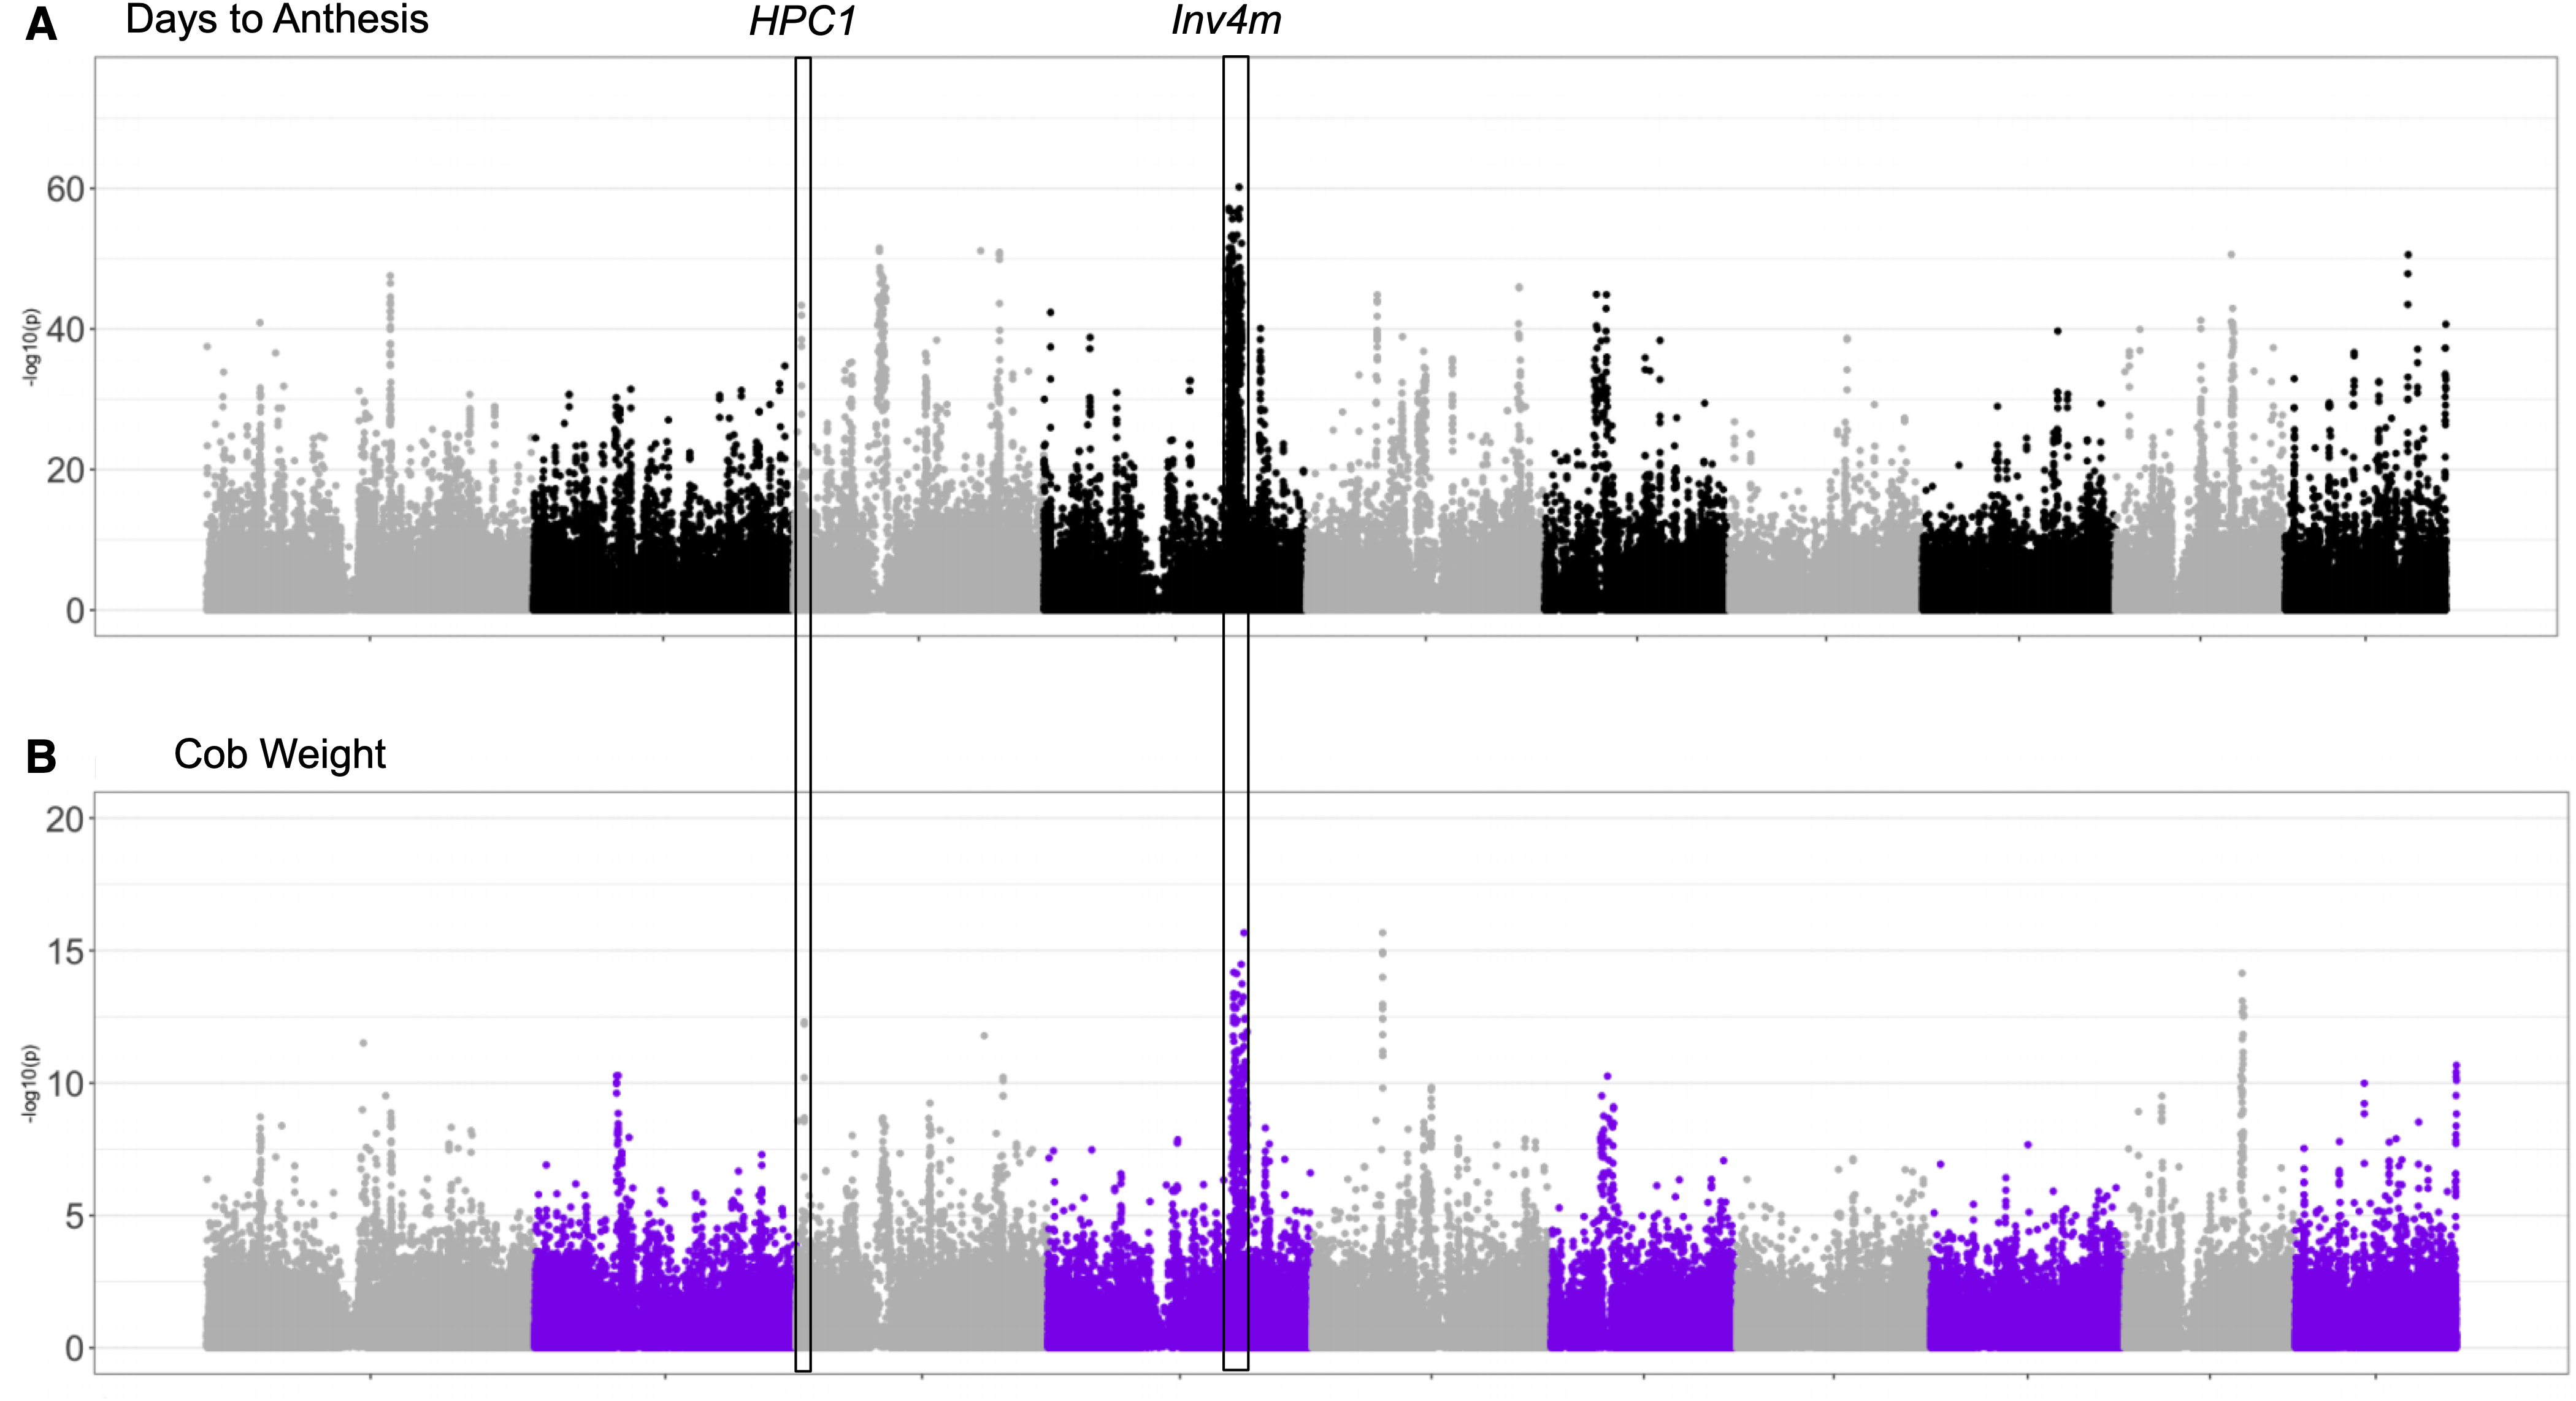
\includegraphics[width=0.8 \paperwidth]{Sup_Figures/Sup_Fig_9.png}
\caption[Genome wide association of genotype by elevation by genotype interactions of days to anthesis.]{Genome wide association of genotype by elevation by genotype interactions of days to anthesis \textbf{(A)} and cob weight \textbf{(B)} using data from \cite{gates2019-xu}}.
\label{figure:Sup:GxE_scan}
\end{center}
\end{figure*} 
\clearpage

\begin{figure*}[t]
\begin{center}
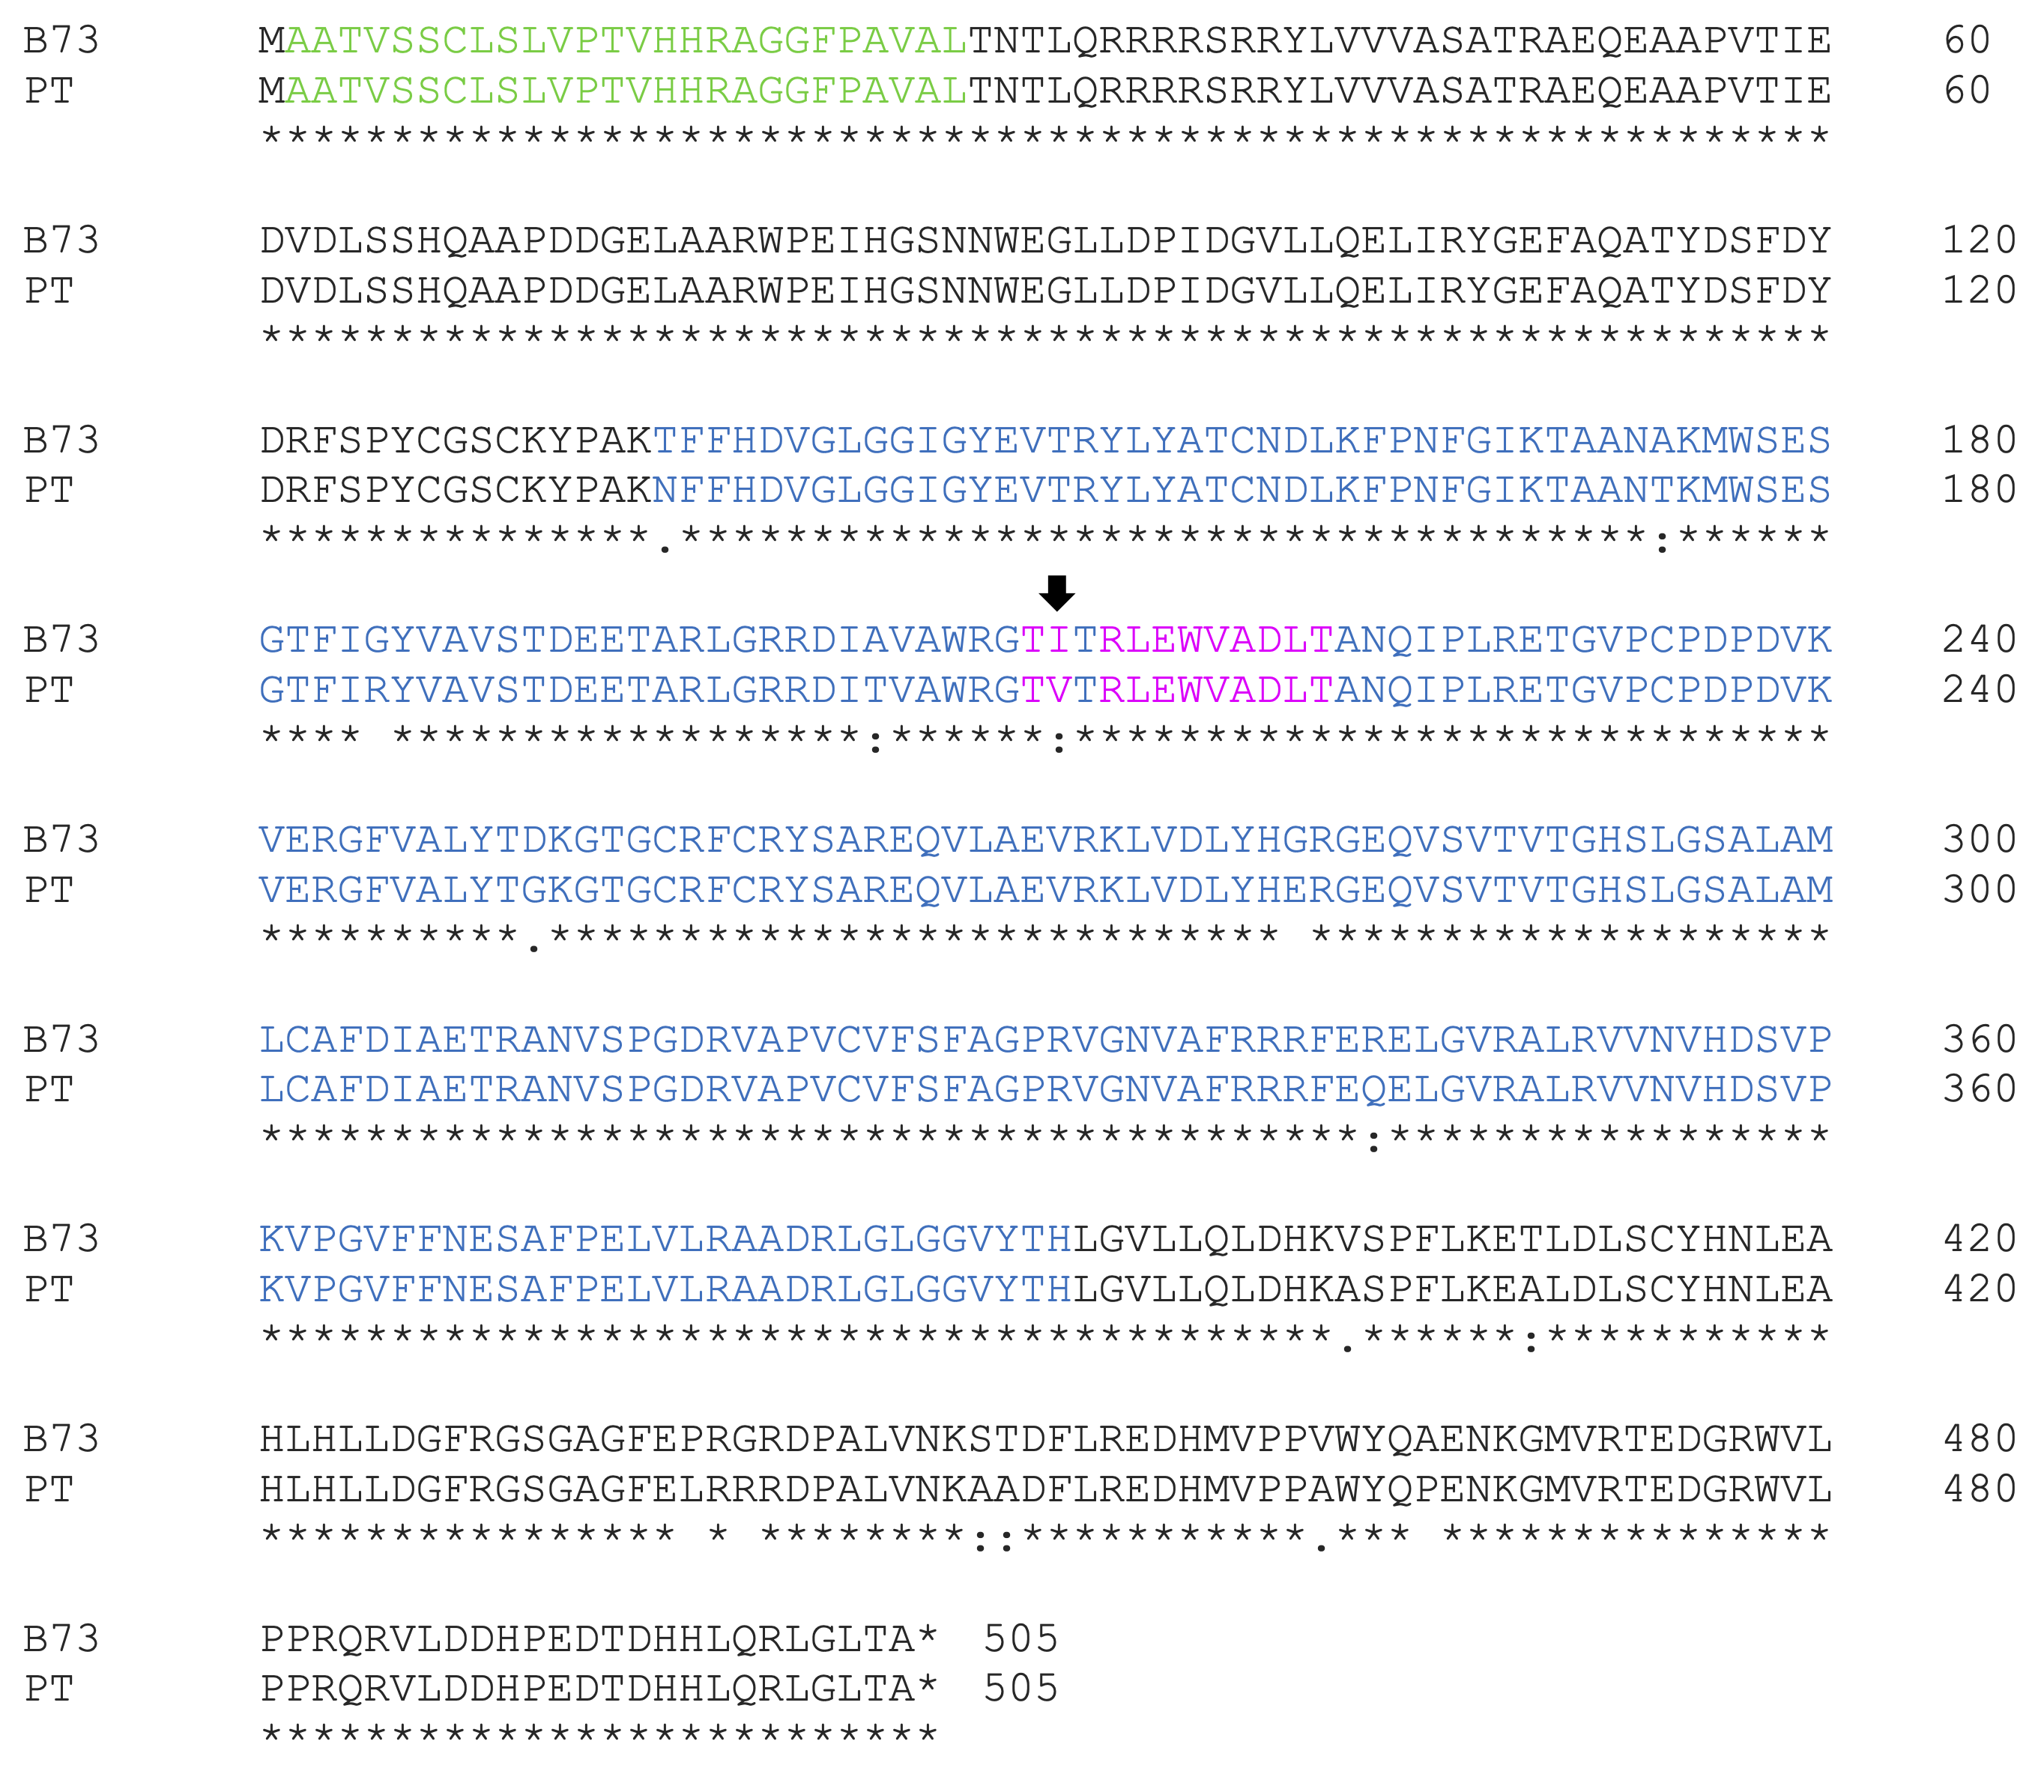
\includegraphics[width=\linewidth]{Sup_Figures/Sup_Fig_10.png}
\caption[Alignment of HPC1-B73 and HPC1-PT.]
{\textbf{Alignment of HPC1-B73 and HPC1-PT.}
Green residues are those from the chloroplast transit peptide.
Blue resides are part of the Lipase3 domain. 
Magenta residues are the flap lid. 
Arrow denotes I211V mutation. “*” denotes matching sequence, “:” denotes conservation between groups with similar properties, “.” denotes conservation of groups with weakly similar properties.
Aminoacid sequence aligned with ClustalOmega.}
\label{figure:Sup:aa_alignment}
\end{center}
\end{figure*} 
\clearpage

\begin{figure*}[t]
\begin{center}
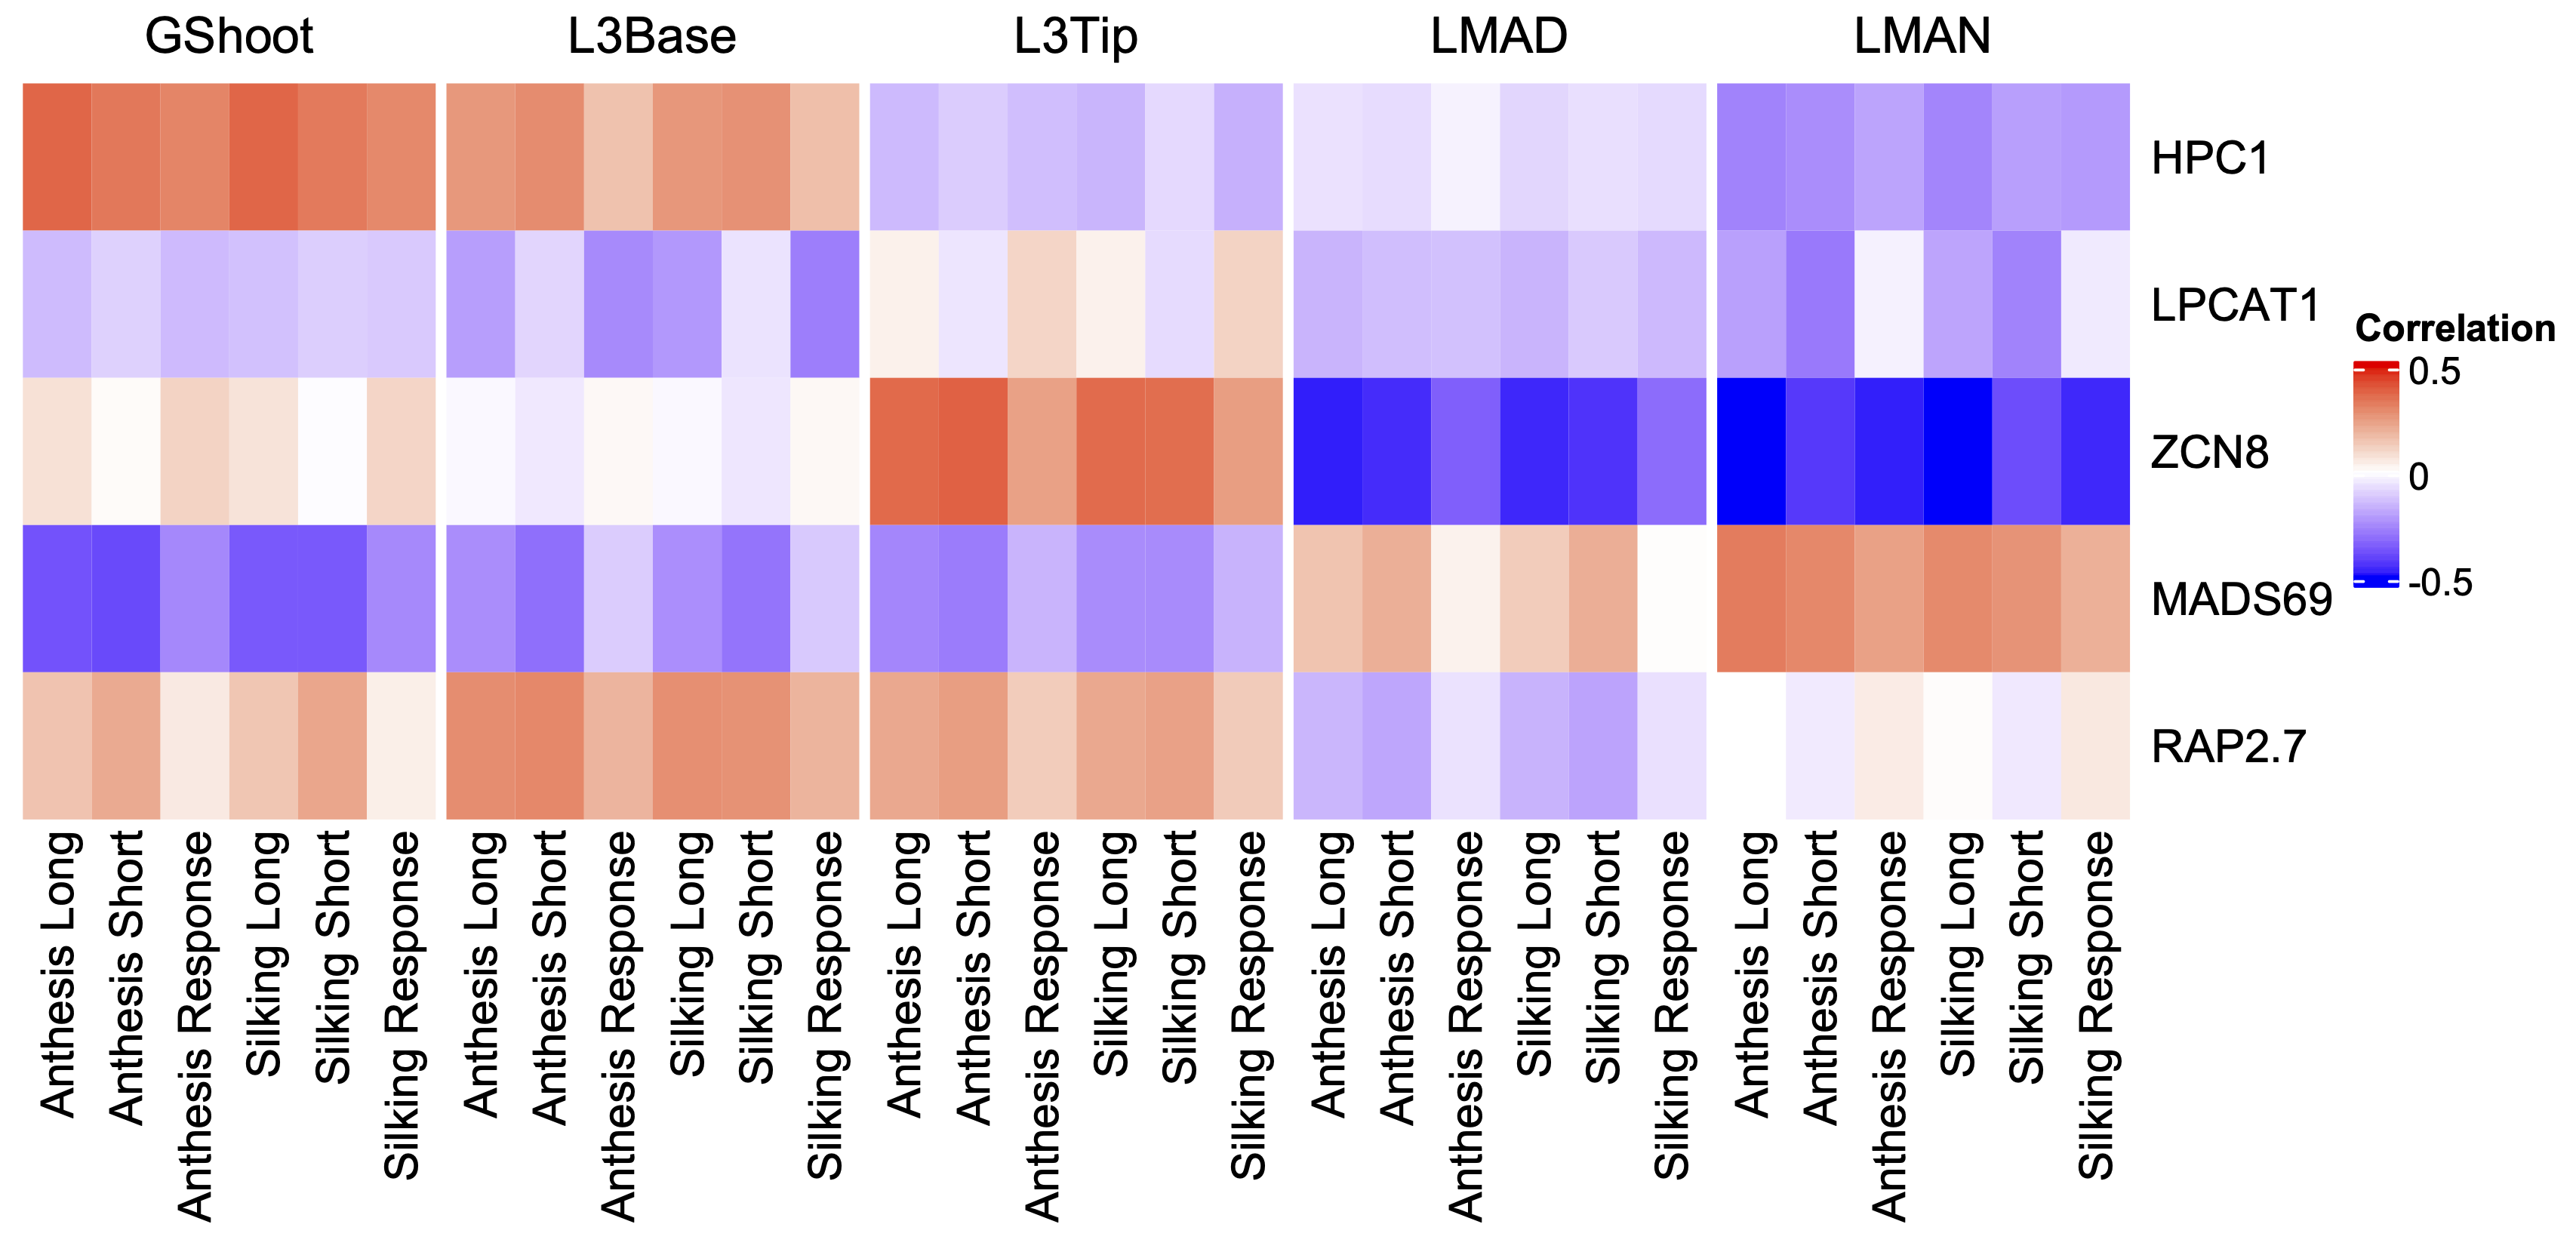
\includegraphics[width=\linewidth]{Sup_Figures/Sup_Fig_11.png}
\caption[Correlation between flowering time and expression of phospholipid-related genes.]
{\textbf{Correlation between flowering time and expression of phospholipid-related genes.} 
Gene expression was correlated to flowering time traits from aerial tissues in the 282 diversity panel. 
Data obtained from \citep{kremling2018-gn}.}
\label{figure:Sup:cor_heatmap}
\end{center}
\end{figure*} 
\clearpage

\begin{figure*}[t]
\begin{center}
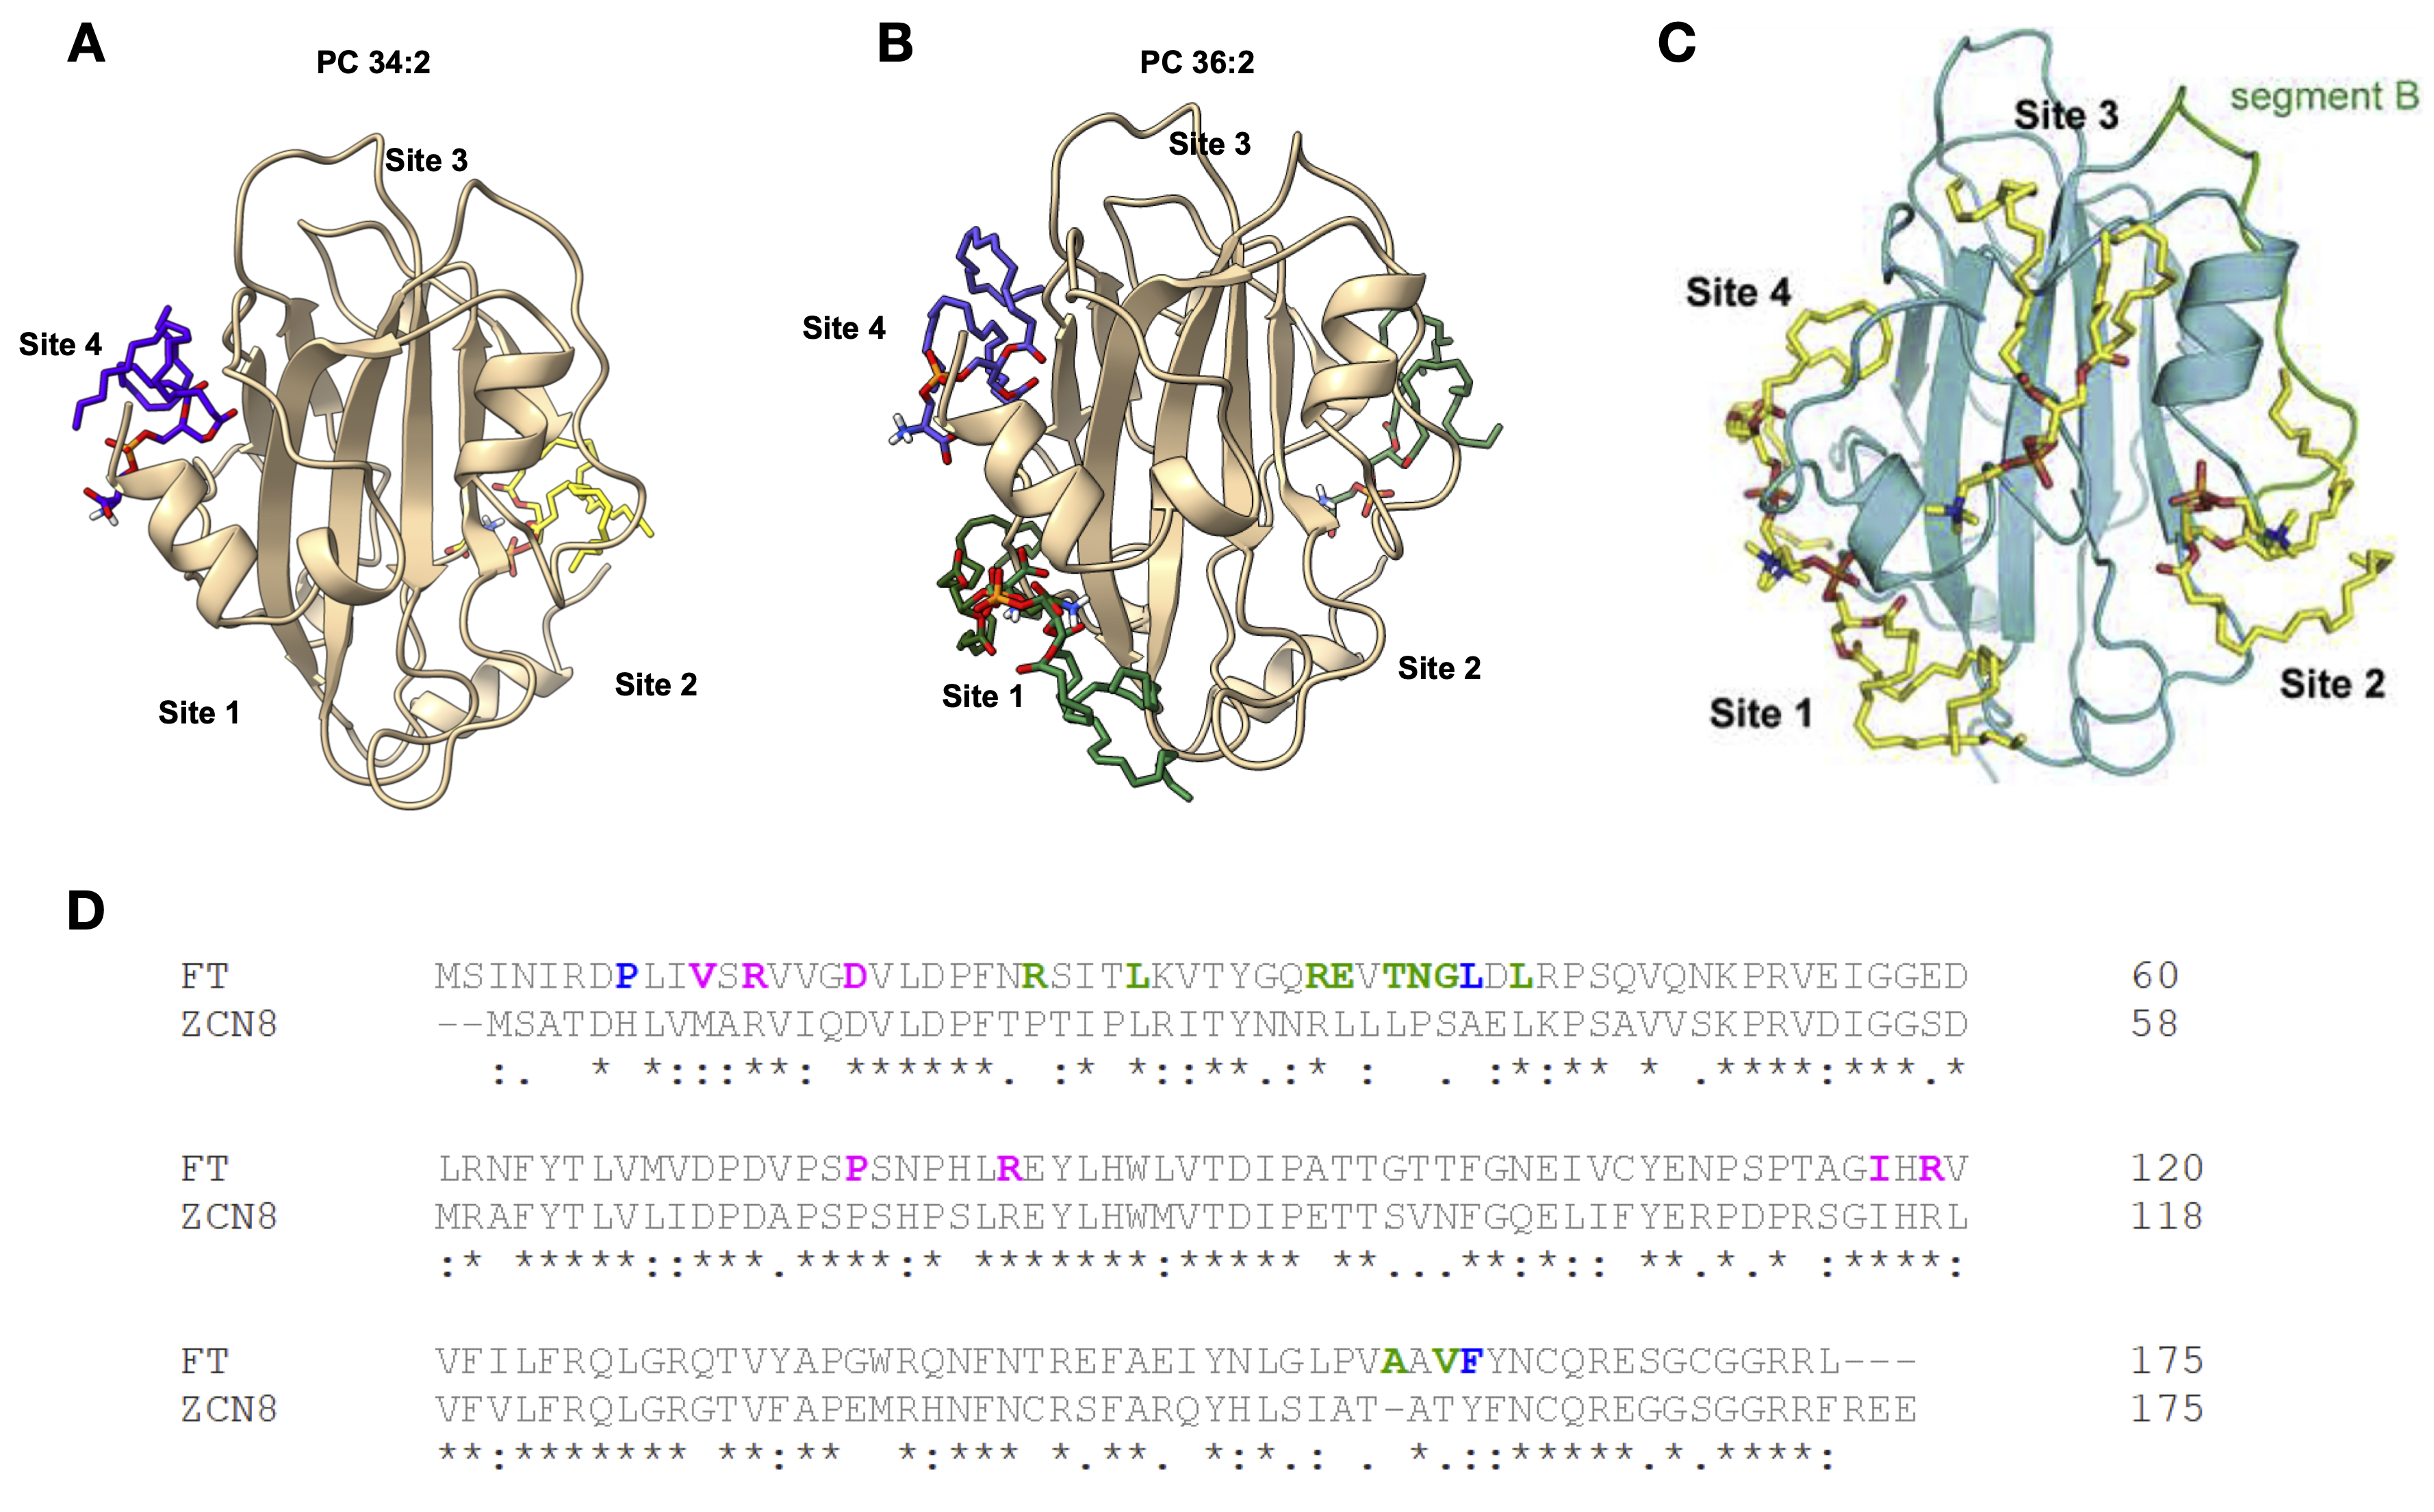
\includegraphics[width=\linewidth]{Sup_Figures/Sup_Fig_12.png}
\caption[Predicted binding sites of ZCN8 align with binding sites of Arabidopsis FT.]
{\textbf{Predicted binding sites of ZCN8 align with binding sites of Arabidopsis FT.}
Shown are AutoDock Vina \cite{trott2010-su} ZCN8 - lipid docking interactions of a RoseTTAFold \cite{baek2021sci} model of ZCN8 PC 34:2 \textbf{(A)} and PC 36:2 \textbf{(B)} compared with the docking model of PC 36:2 \textit{Arabidopsis thaliana} FT \textbf{(C)} from \cite{nakamura2019-ht}. 
Docking was performed on an NMRBox server \cite{maciejewski2010bj}.
\textbf{(D)} Alignment of \textit{Arabidopsis thaliana} FT and \textit{Zea mays} ZCN8. 
Residues in blue are present in both docking site 1 and docking site 4 identified in \cite{nakamura2019-ht}. 
Residues in magenta are present only in docking site 1 while residues in green are present only in docking site 4. 
Symbols below the residues indicate level of alignment where * denotes complete alignment, : represents a conserved substitution, and . represents a semi-conserved substitution.}
\label{figure:Sup:Docking}
\end{center}
\end{figure*} 


\begin{figure*}[t]
\begin{center}
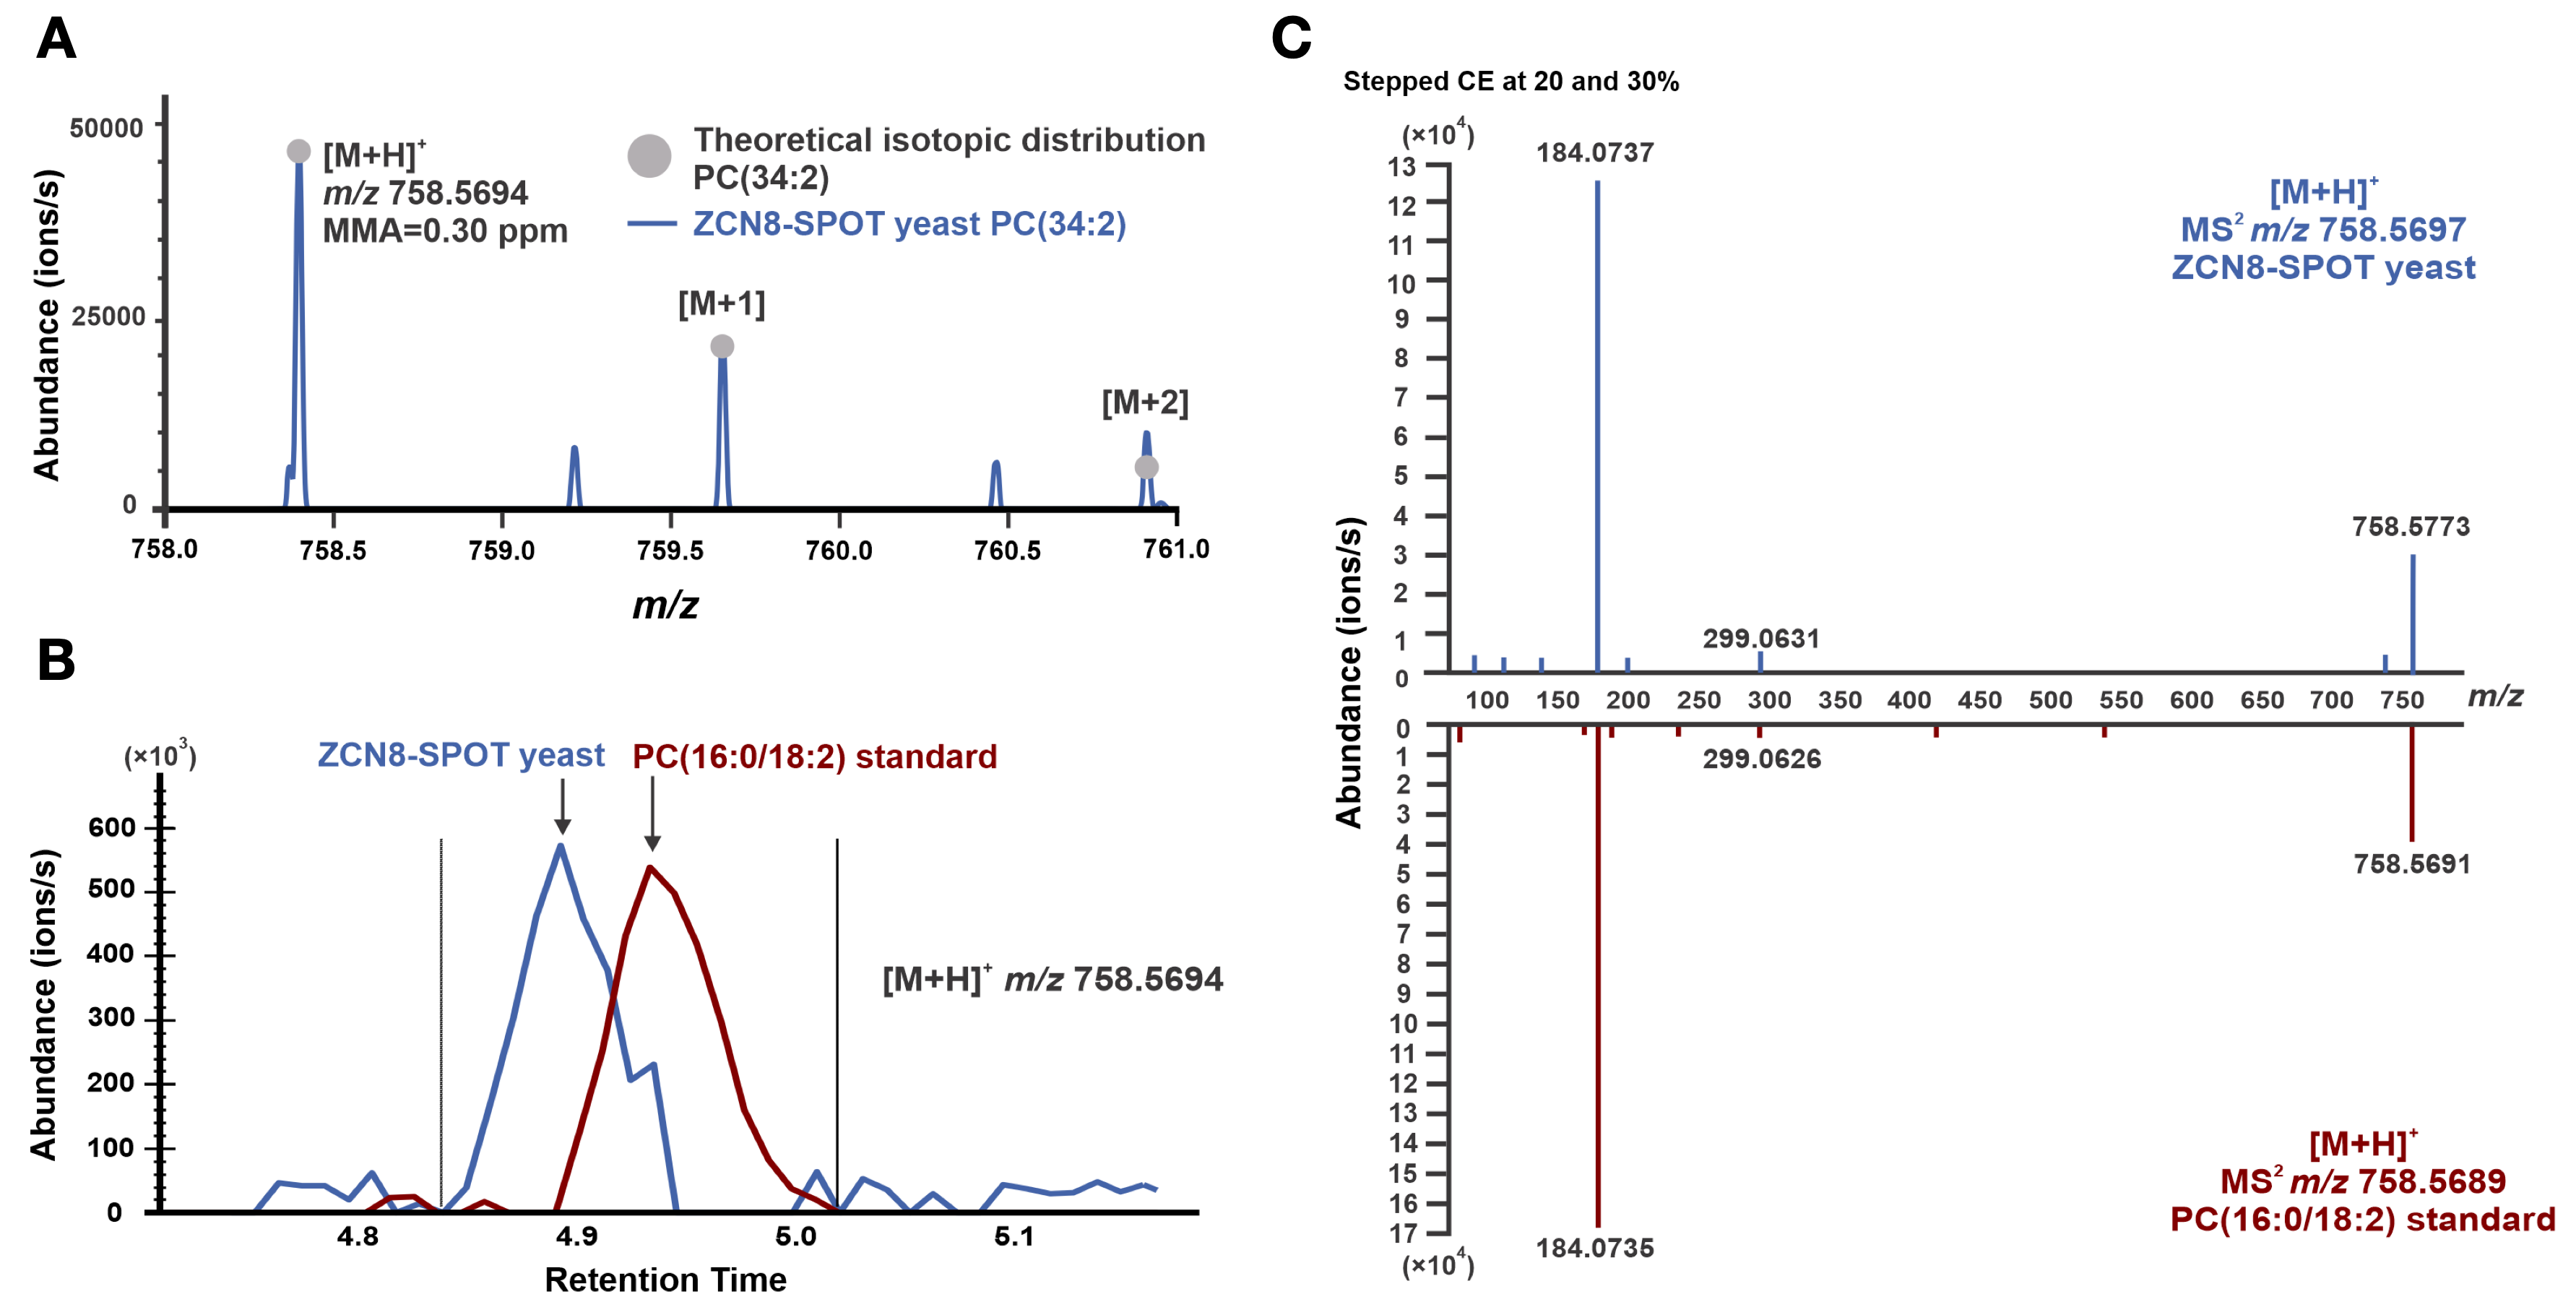
\includegraphics[width=\linewidth]{Sup_Figures/Sup_Fig_14.png}
\caption[ZCN8 binds to phosphatidylcholine.]
{ \textbf{ZCN8 binds to phosphatidylcholine}.
\textbf{(A)} Mass spectrum of ZCN8-SPOT yeast sample compared to the theoretical isotopic pattern of PC(34:2) at [M+H]\textsuperscript{+} \textit{m/z} 758.5694. The experimental \textit{m/z} and mass measurement accuracy (MMA) are labeled. The spectrum of ZCN8-SPOT is an average of 16 scans across the chromatographic peak of \textit{m/z} 758.5694.  
\textbf{(B)} Extracted ion chromatogram of \textit{m/z} 758.5694 from the PC(16:0/18:2) standard and ZCN8-SPOT yeast from two separate injections.  
\textbf{(C)s} MS\textsuperscript{2} fragmentation spectra comparison for \textit{m/z} 758.5694 from ZCN8-SPOT yeast and the PC(16:0/18:2) standard.
The comparison data between an authentic standard and ZCN8-SPOT yeast was acquired with the same lipid profiling method as described in the Materials and Methods section for the Thermo Scientific Orbitrap Exploris 480 mass spectrometer with the following modifications:  the injection volume was 10 $\mu$L, full scan spectra were acquired from \textit{m/z} 200 – 1000 and \textit{m/z} 758.5694 was included in the target mass
list for MS\textsuperscript{2} selection.}
\label{figure:Sup:ZCN8-PC}
\end{center}
\end{figure*}


